为了了解移动语义的基本原则,使用小段代码为例,首先没有移动语义(例如,用一个旧的C++编译器编译,仅支持C++03),之后再用移动语义(用现代C++编译器编译,支持C++11或更高的版本)。\par

\hspace*{\fill} \par %插入空行
\textbf{C++03的示例(使用移动语义之前)}

假设我们有以下代码:\par

{\color{red}{basics/motiv03.cpp}}

\begin{lstlisting}[caption={}]
#include <string>
#include <vector>

std::vector<std::string> createAndInsert()
{
	std::vector<std::string> coll; // create vector of strings
	coll.reserve(3); // reserve memory for 3 elements
	std::string s = "data"; // create string object
	
	coll.push_back(s); // insert string object
	coll.push_back(s+s); // insert temporary string
	coll.push_back(s); // insert string
	
	return coll; // return vector of strings
}

int main()
{
	std::vector<std::string> v; // create empty vector of strings
	...
	v = createAndInsert(); // assign returned vector of strings
	...
}
\end{lstlisting}

使用不支持移动语义的C++编译器编译这段代码后,让我们看一下程序执行的各个步骤(检查堆栈和堆)。\par

\begin{itemize}
	\item 首先,在main()中,我们创建了空的vector \textit{v}:\par
	\textit{\textbf{std::vector<std::string> v;}} \par
	存放在堆栈上,元素数为0,未为元素分配内存。
	\item 然后,调用\par
	\textit{\textbf{v = createAndInsert();}}\par
	在堆栈上创建另一个vector \textit{coll},并在堆上为三个元素预留内存:\par
	\textit{\textbf{std::vector<std::string> coll;}}\par
	\textit{\textbf{coll.reserve(3);}}\par
	因为分配的内存没有初始化,所以元素的数量仍然是0。
	\item 然后,用“data”初始化字符串:\par
	\textit{\textbf{std::string s = "data";}}\par
	字符串类似于具有\textit{char}元素的vector。其实是在堆栈上创建一个对象,其中一个成员表示字符的数量(值为4),另一个指针表示字符的内存。\par
	之后,程序的状态如下:堆栈上有三个对象:\textit{v}、\textit{coll}和\textit{s}。其中\textit{coll}和\textit{s}已经在堆上分配了内存:\par
	\begin{center}
		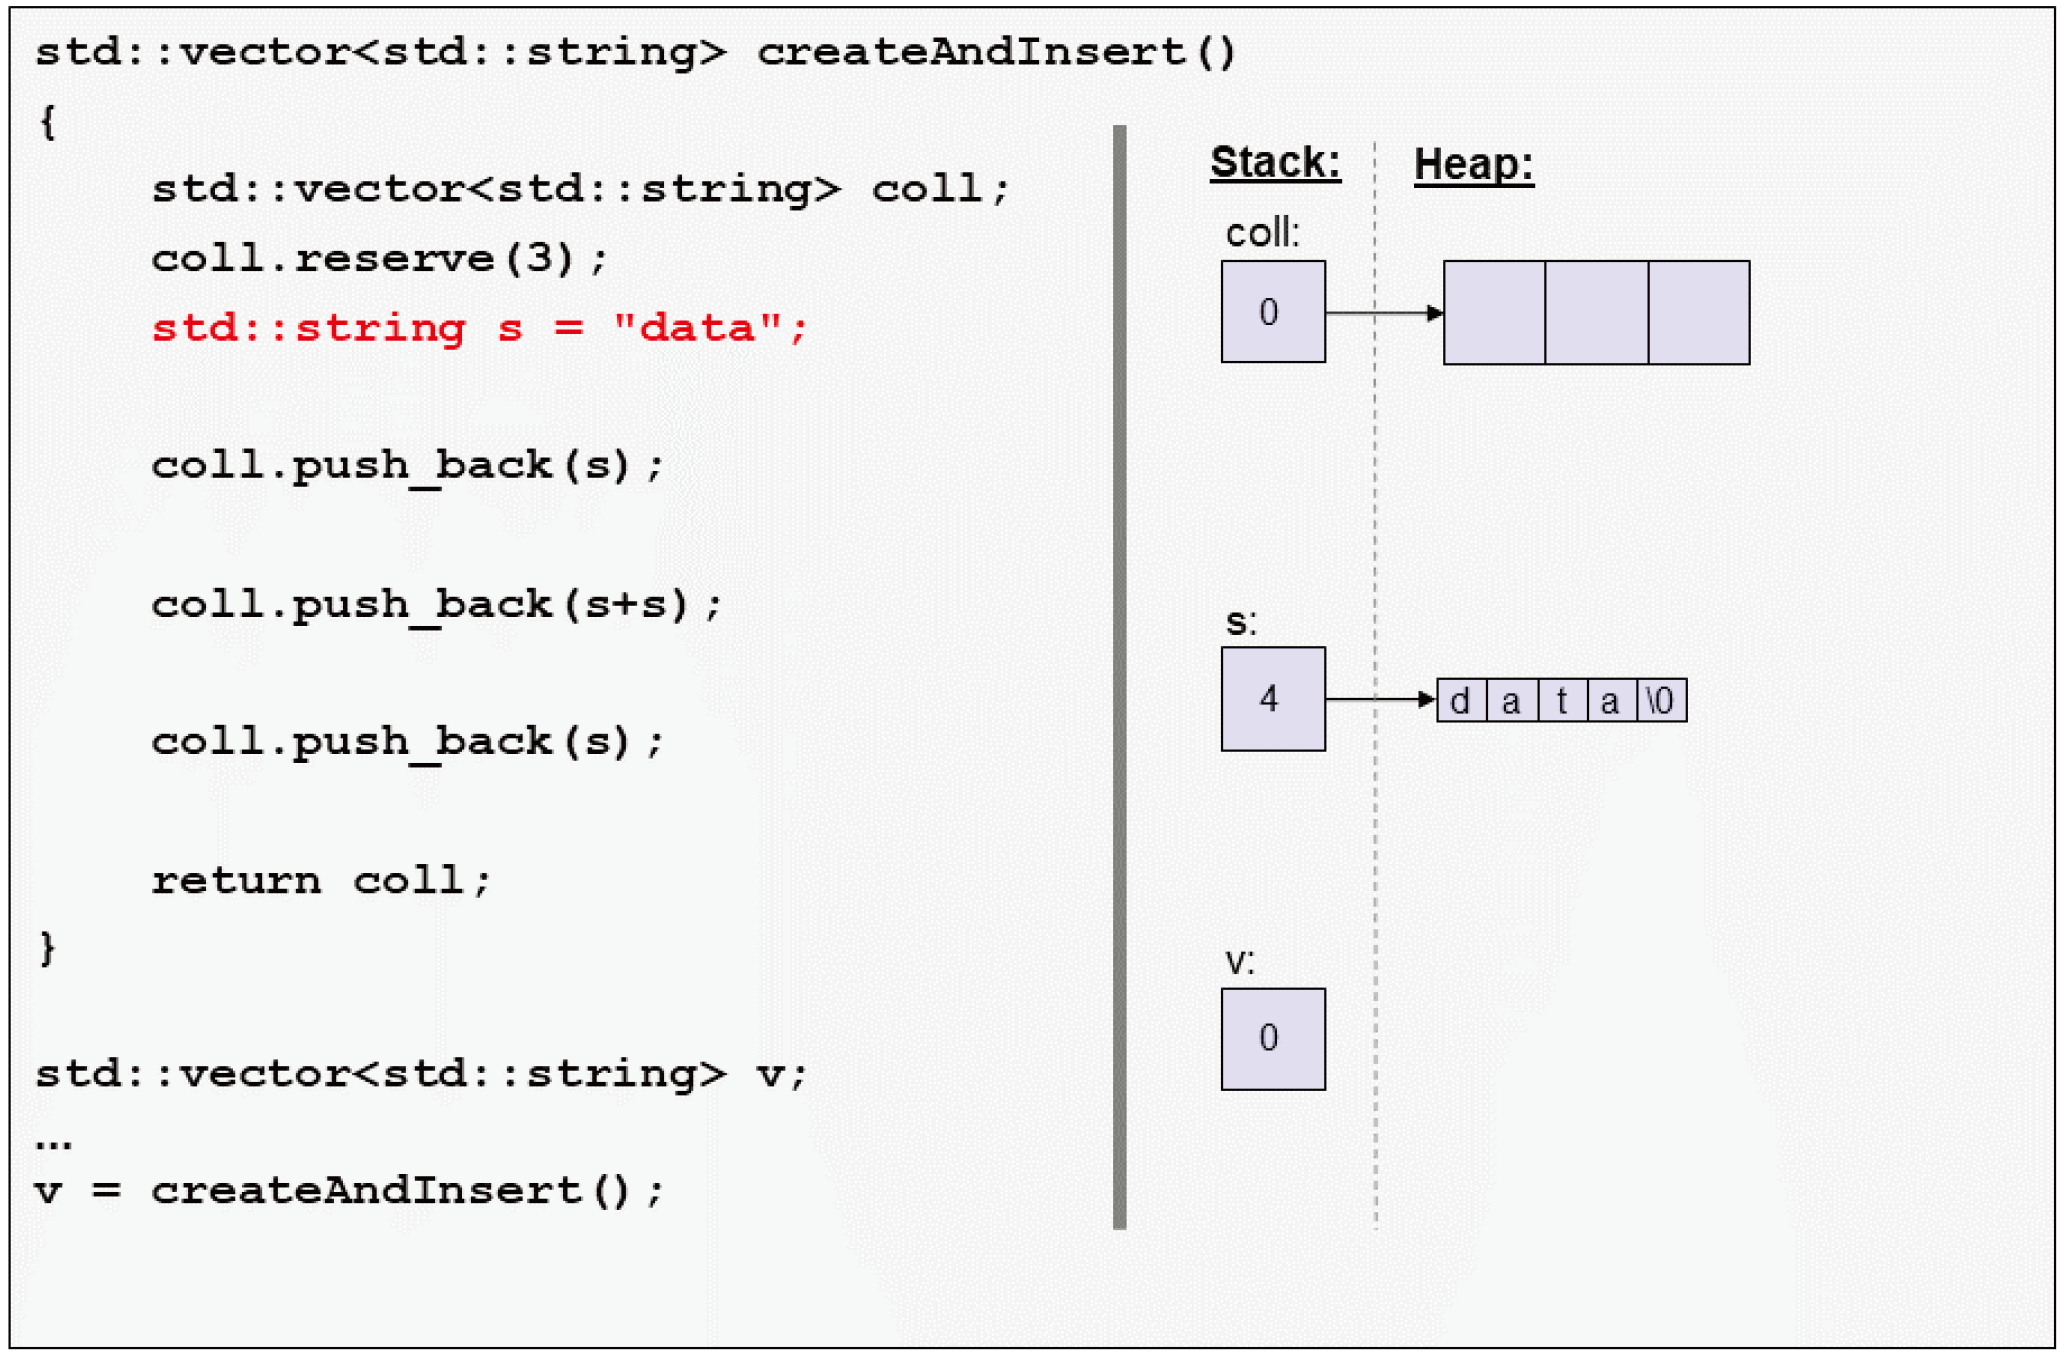
\includegraphics[width=1.0\textwidth]{content/1/chapter1/images/1}
	\end{center}
	\item 下一步是将字符串放到\textit{coll}中:\par
	\textbf{\textit{coll.push\_back(s);}}\par
	C++标准库中的所有容器都具有语义,能创建副本。所以,vector有了第一个元素,它是\textit{s}的副本:\par
	\begin{center}
		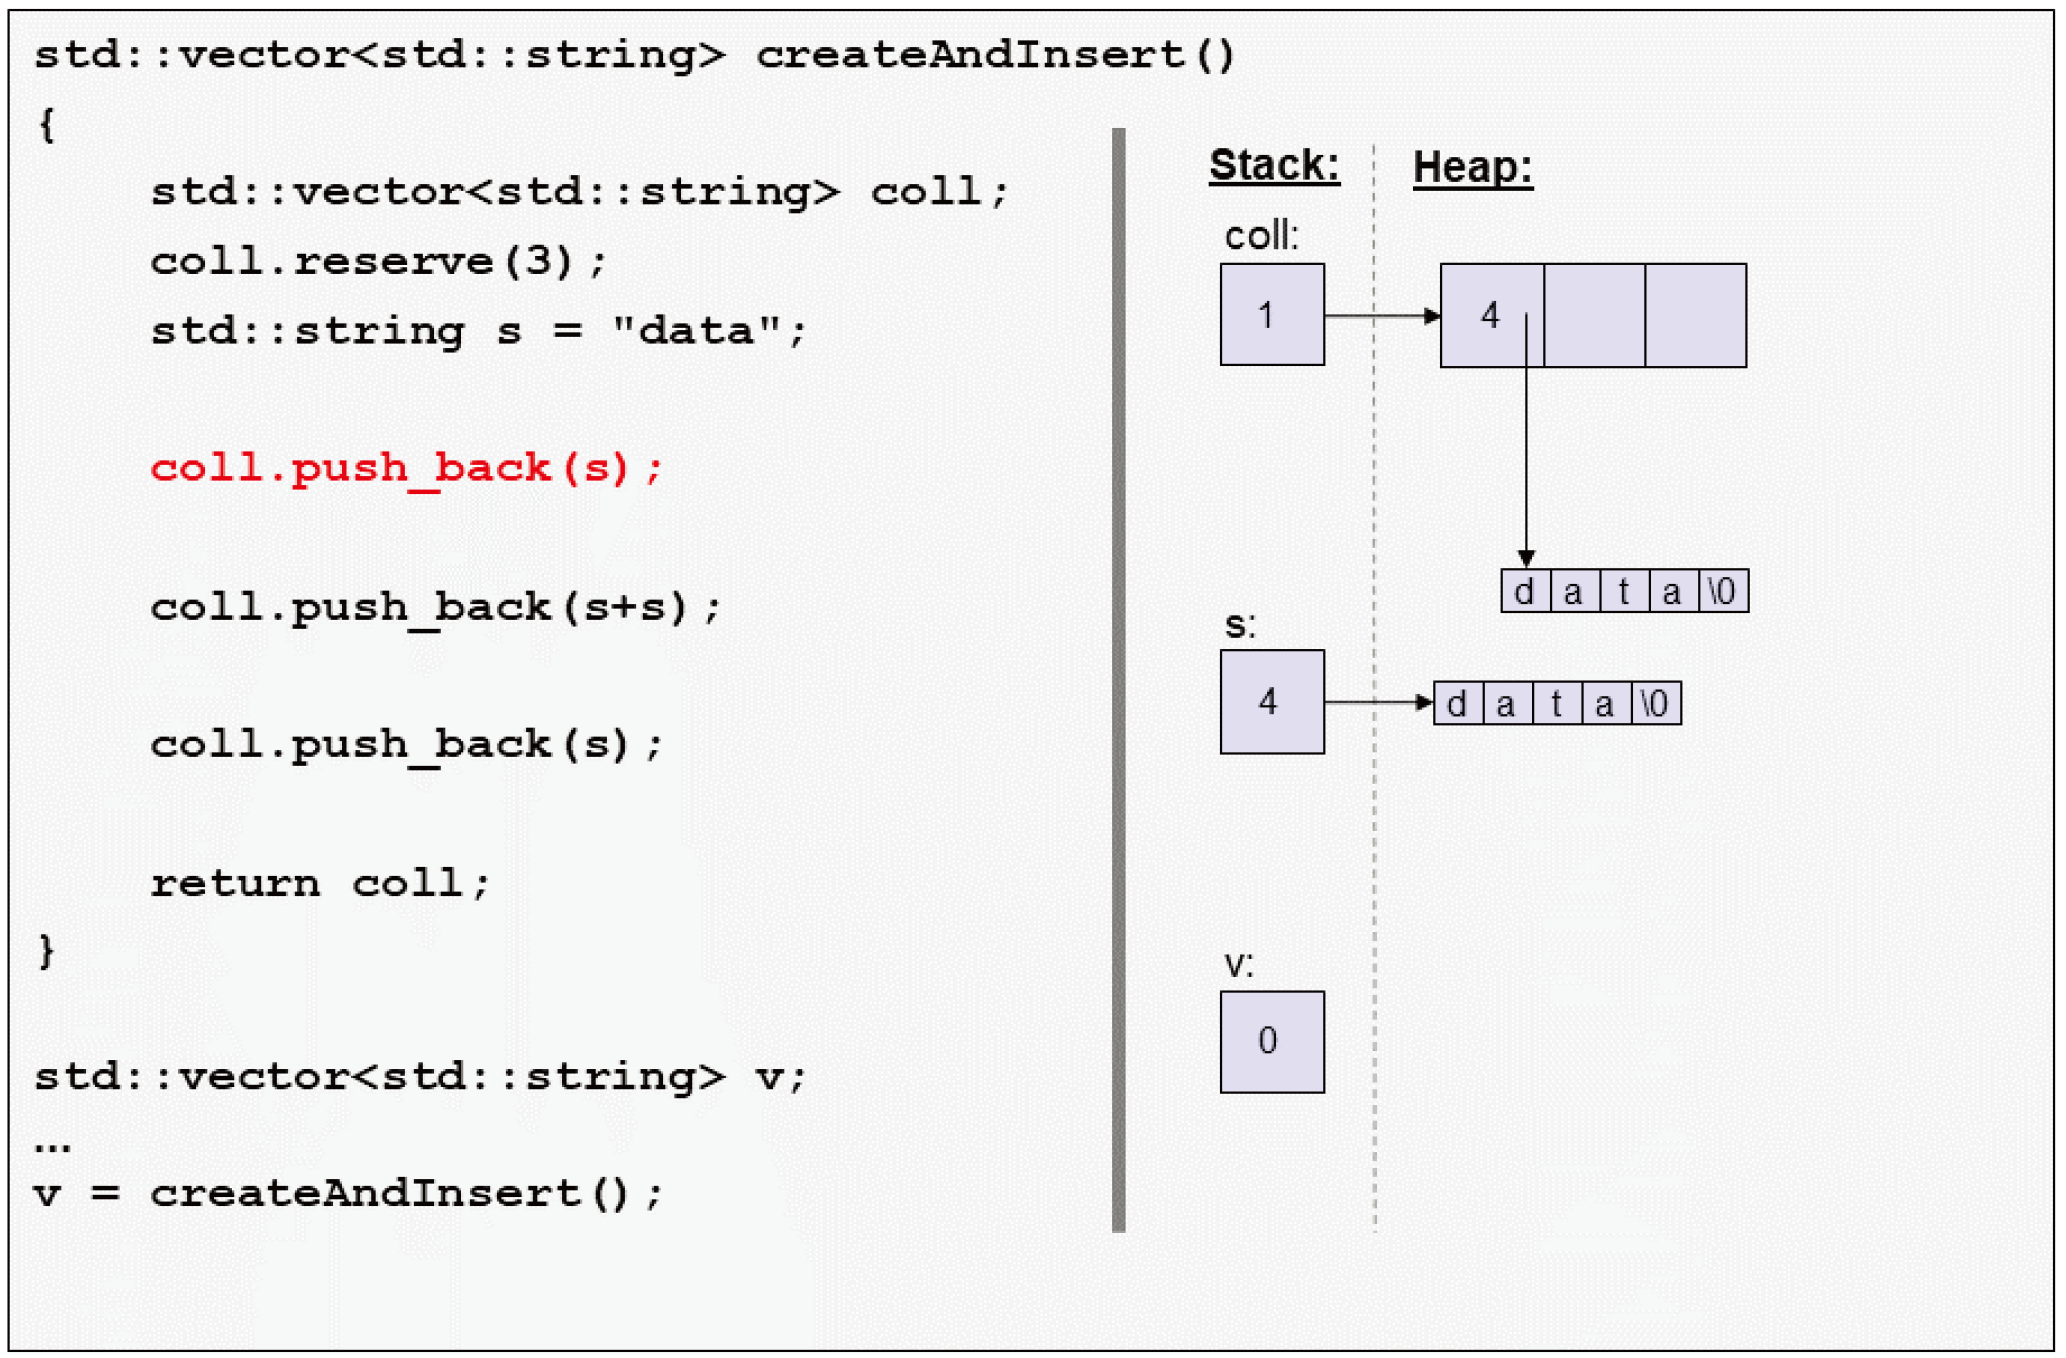
\includegraphics[width=1.0\textwidth]{content/1/chapter1/images/2}
	\end{center}
	目前为止,我们还没有对这个程序中进行优化。现在,我们有两个向量,\textit{v}和\textit{coll},以及两个字符串,\textit{s}和它的副本,这也是\textit{coll}的第一个元素。它们都是独立的对象,有自己的内存。\par
	\item 现在让我们看看下一句,创建了一个新的临时字符串,并再次将其插入vector中:\par
	\textbf{\textit{coll.push\_back(s+s);}}\par
	该语句分三个步骤执行:\par
	\begin{enumerate}
		\item 创建临时字符串s+s:\par
		\begin{center}
			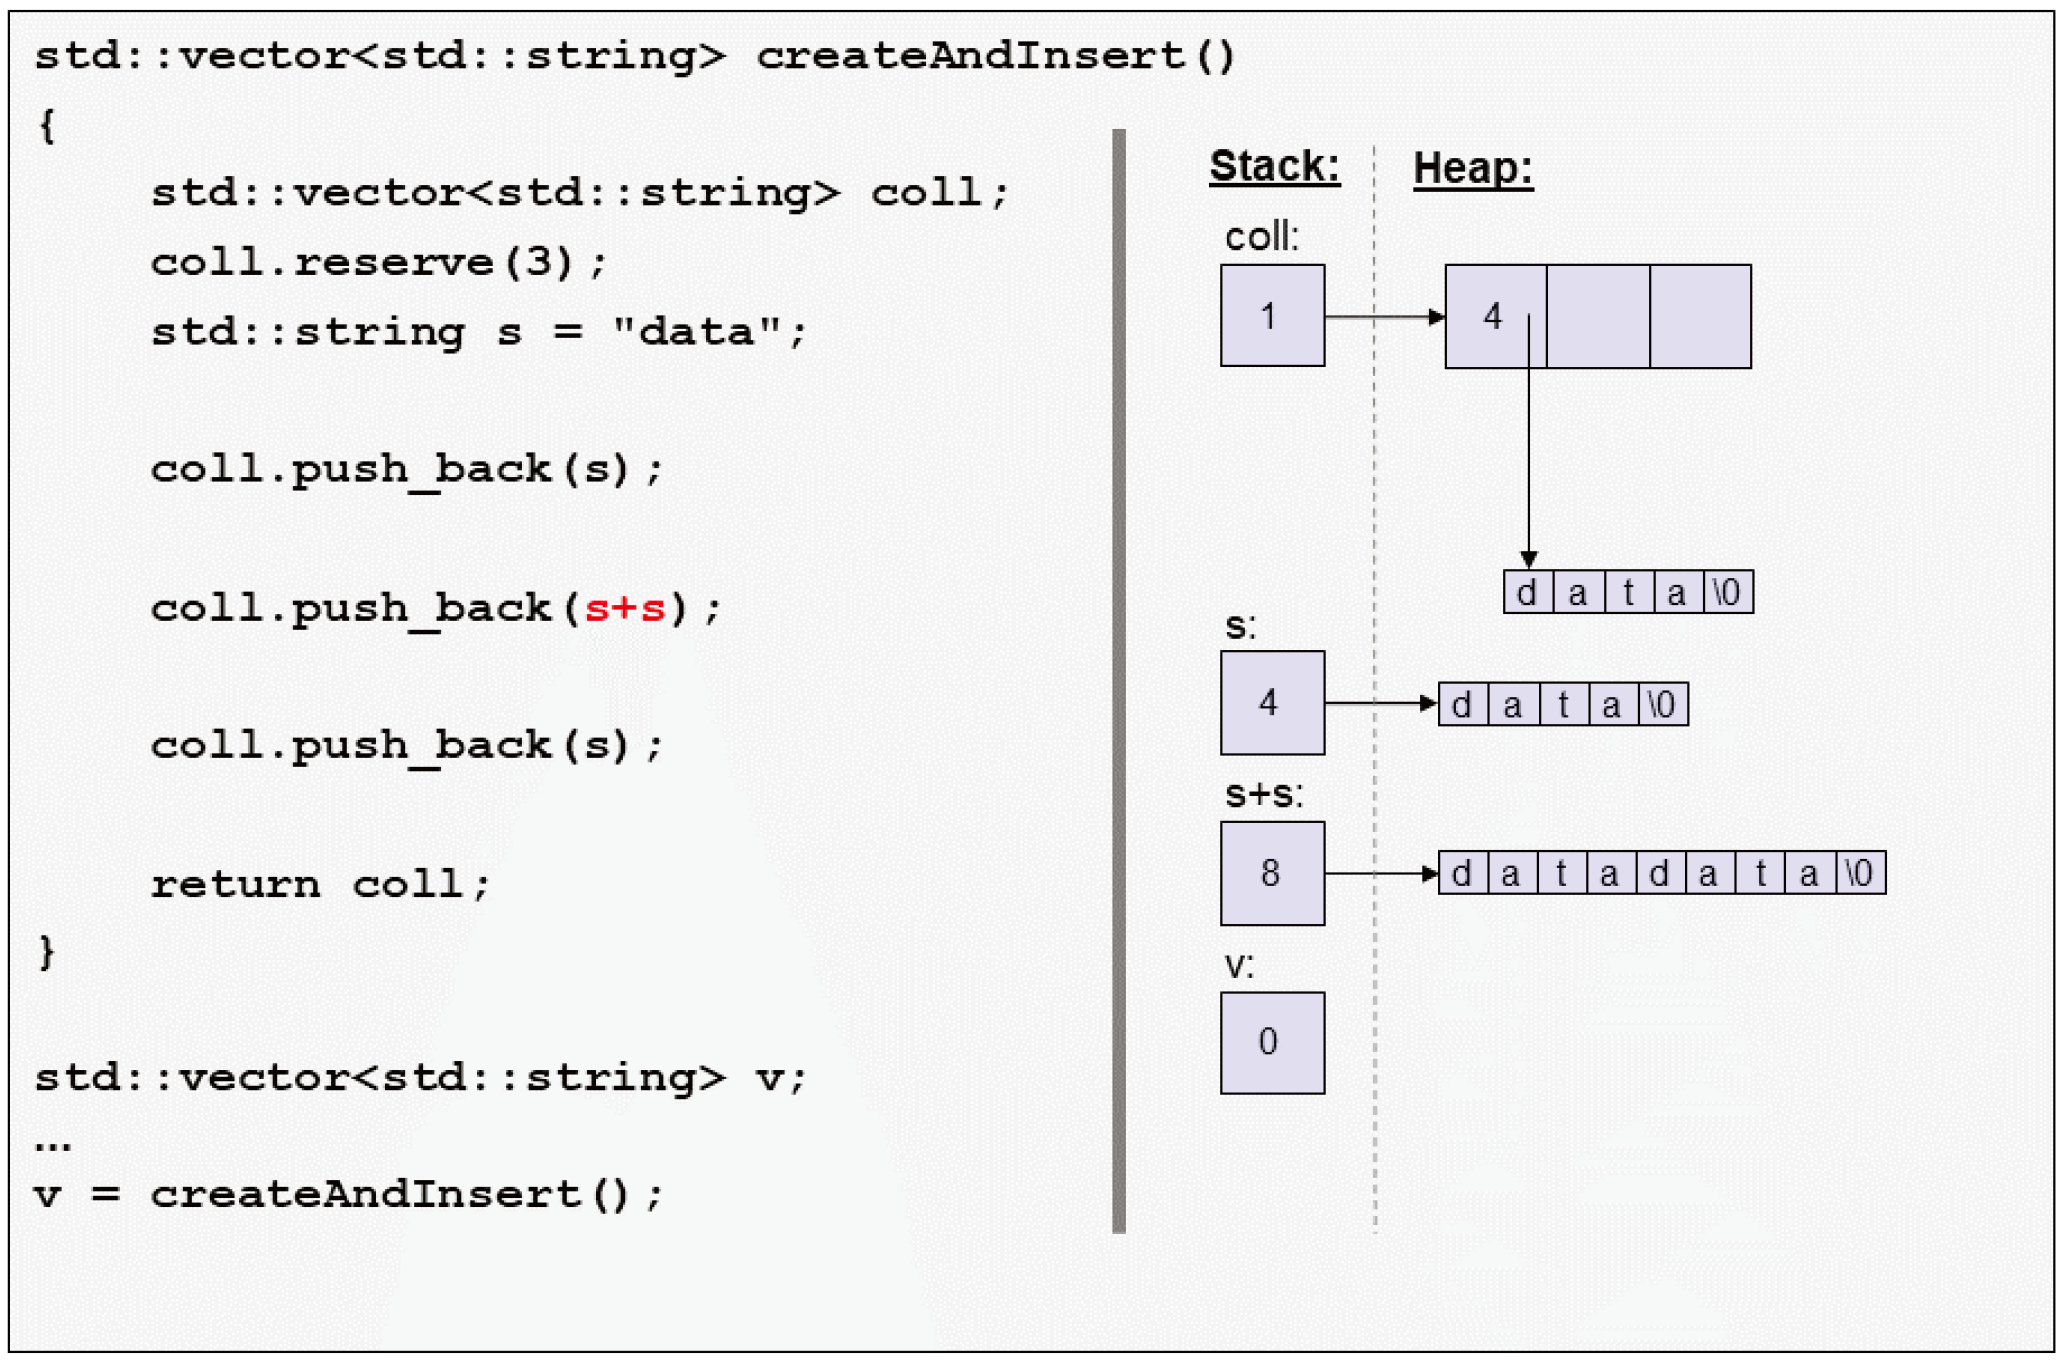
\includegraphics[width=1.0\textwidth]{content/1/chapter1/images/3}
		\end{center}
		\item 将这个临时字符串插入到\textit{coll}中。容器创建副本,创建临时字符串的深层副本,包括分配内存:\par
		\begin{center}
			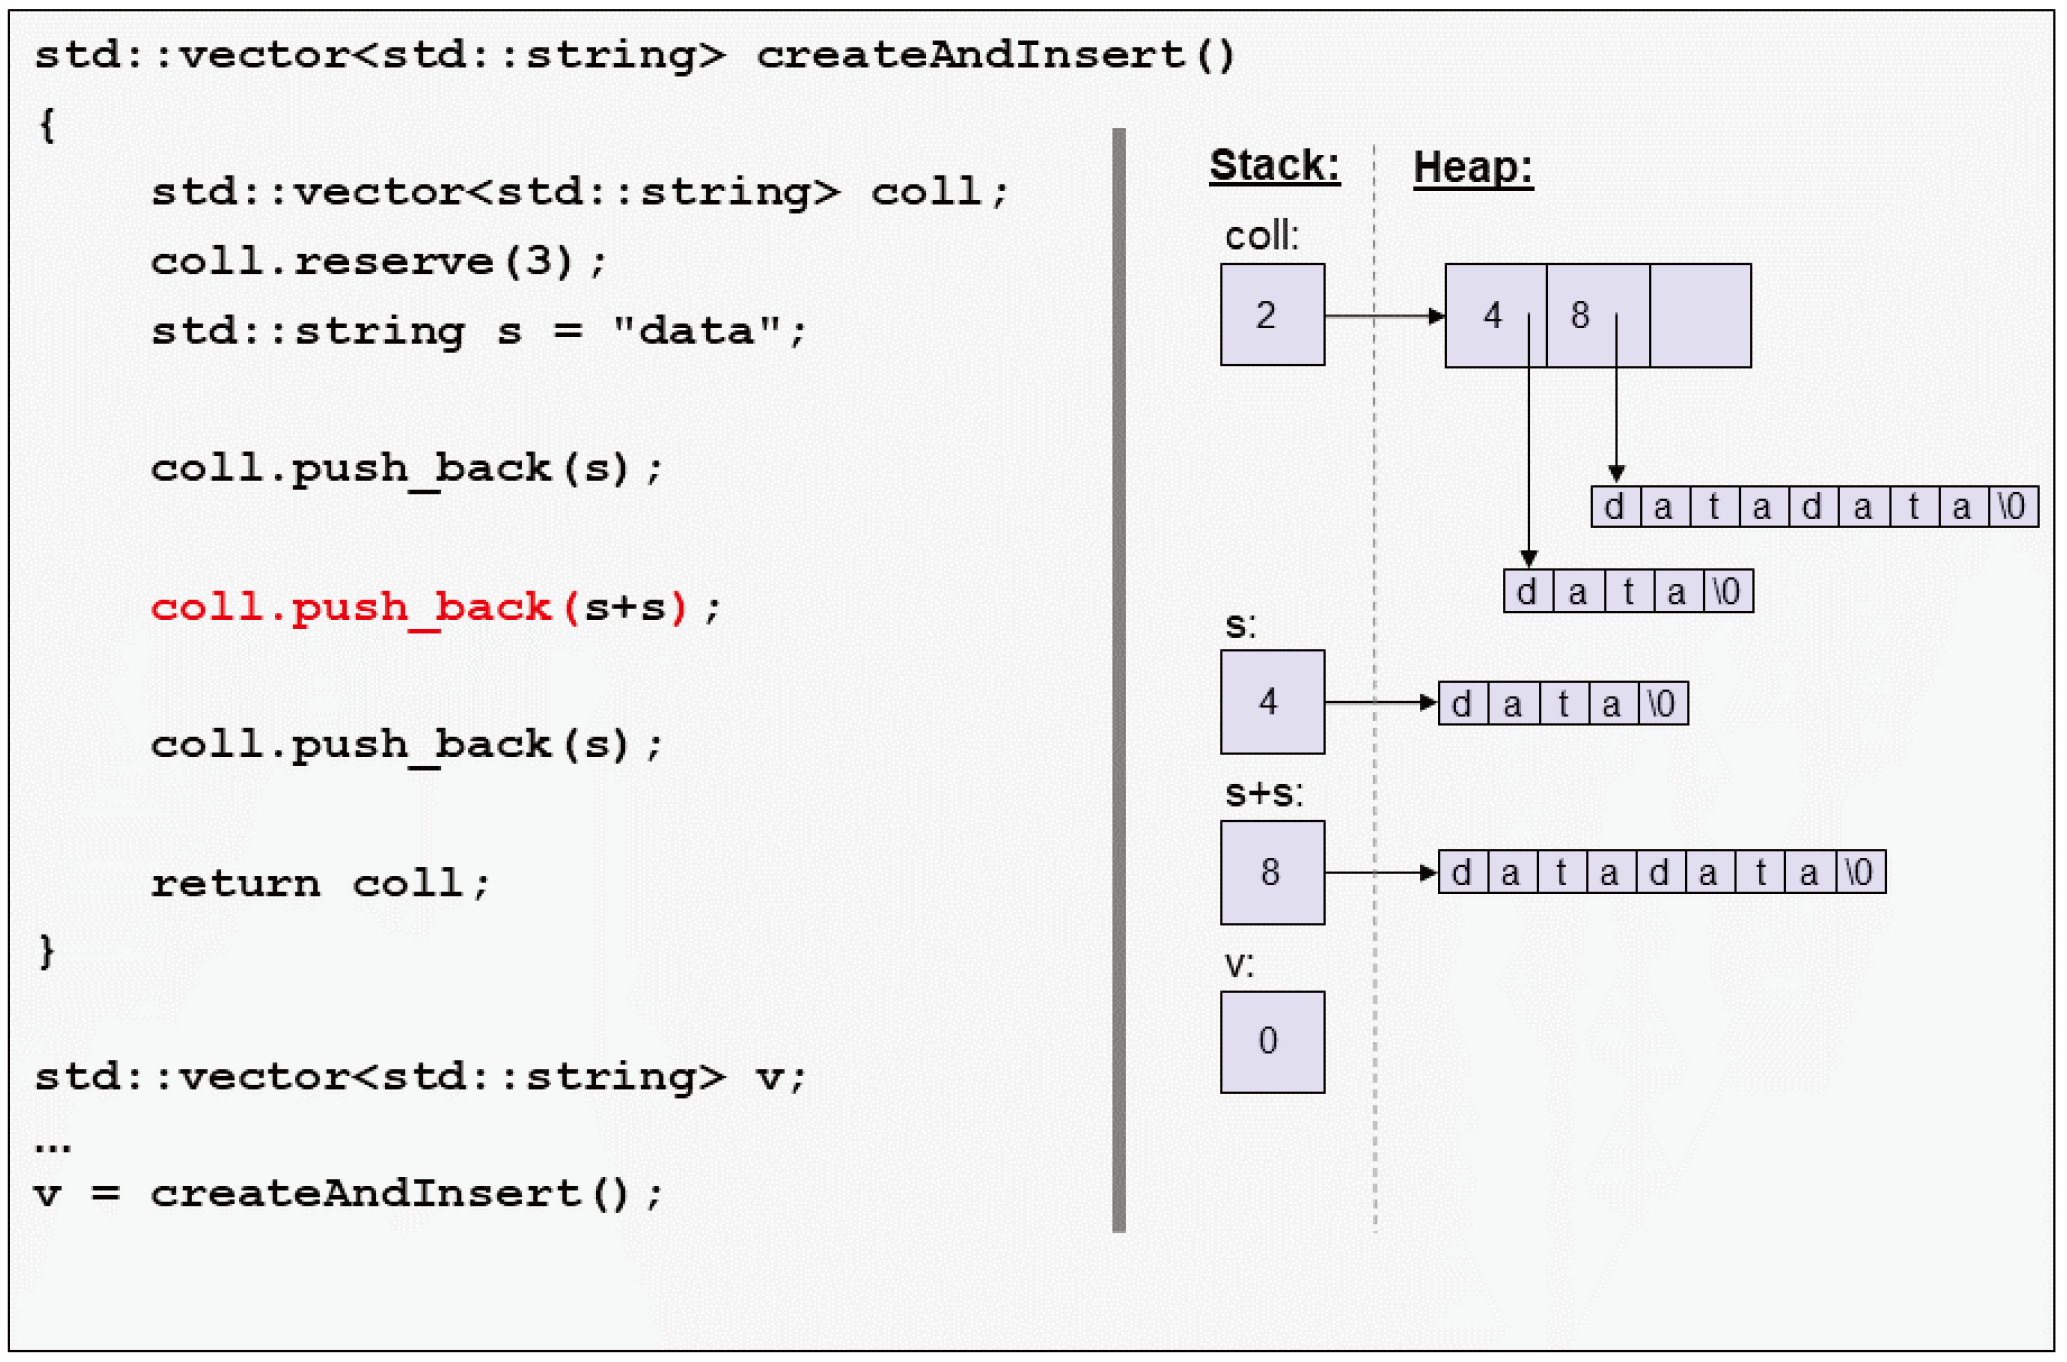
\includegraphics[width=1.0\textwidth]{content/1/chapter1/images/4}
		\end{center}
		\item 末尾,临时字符串\textit{s+s}销毁:\par
		\begin{center}
			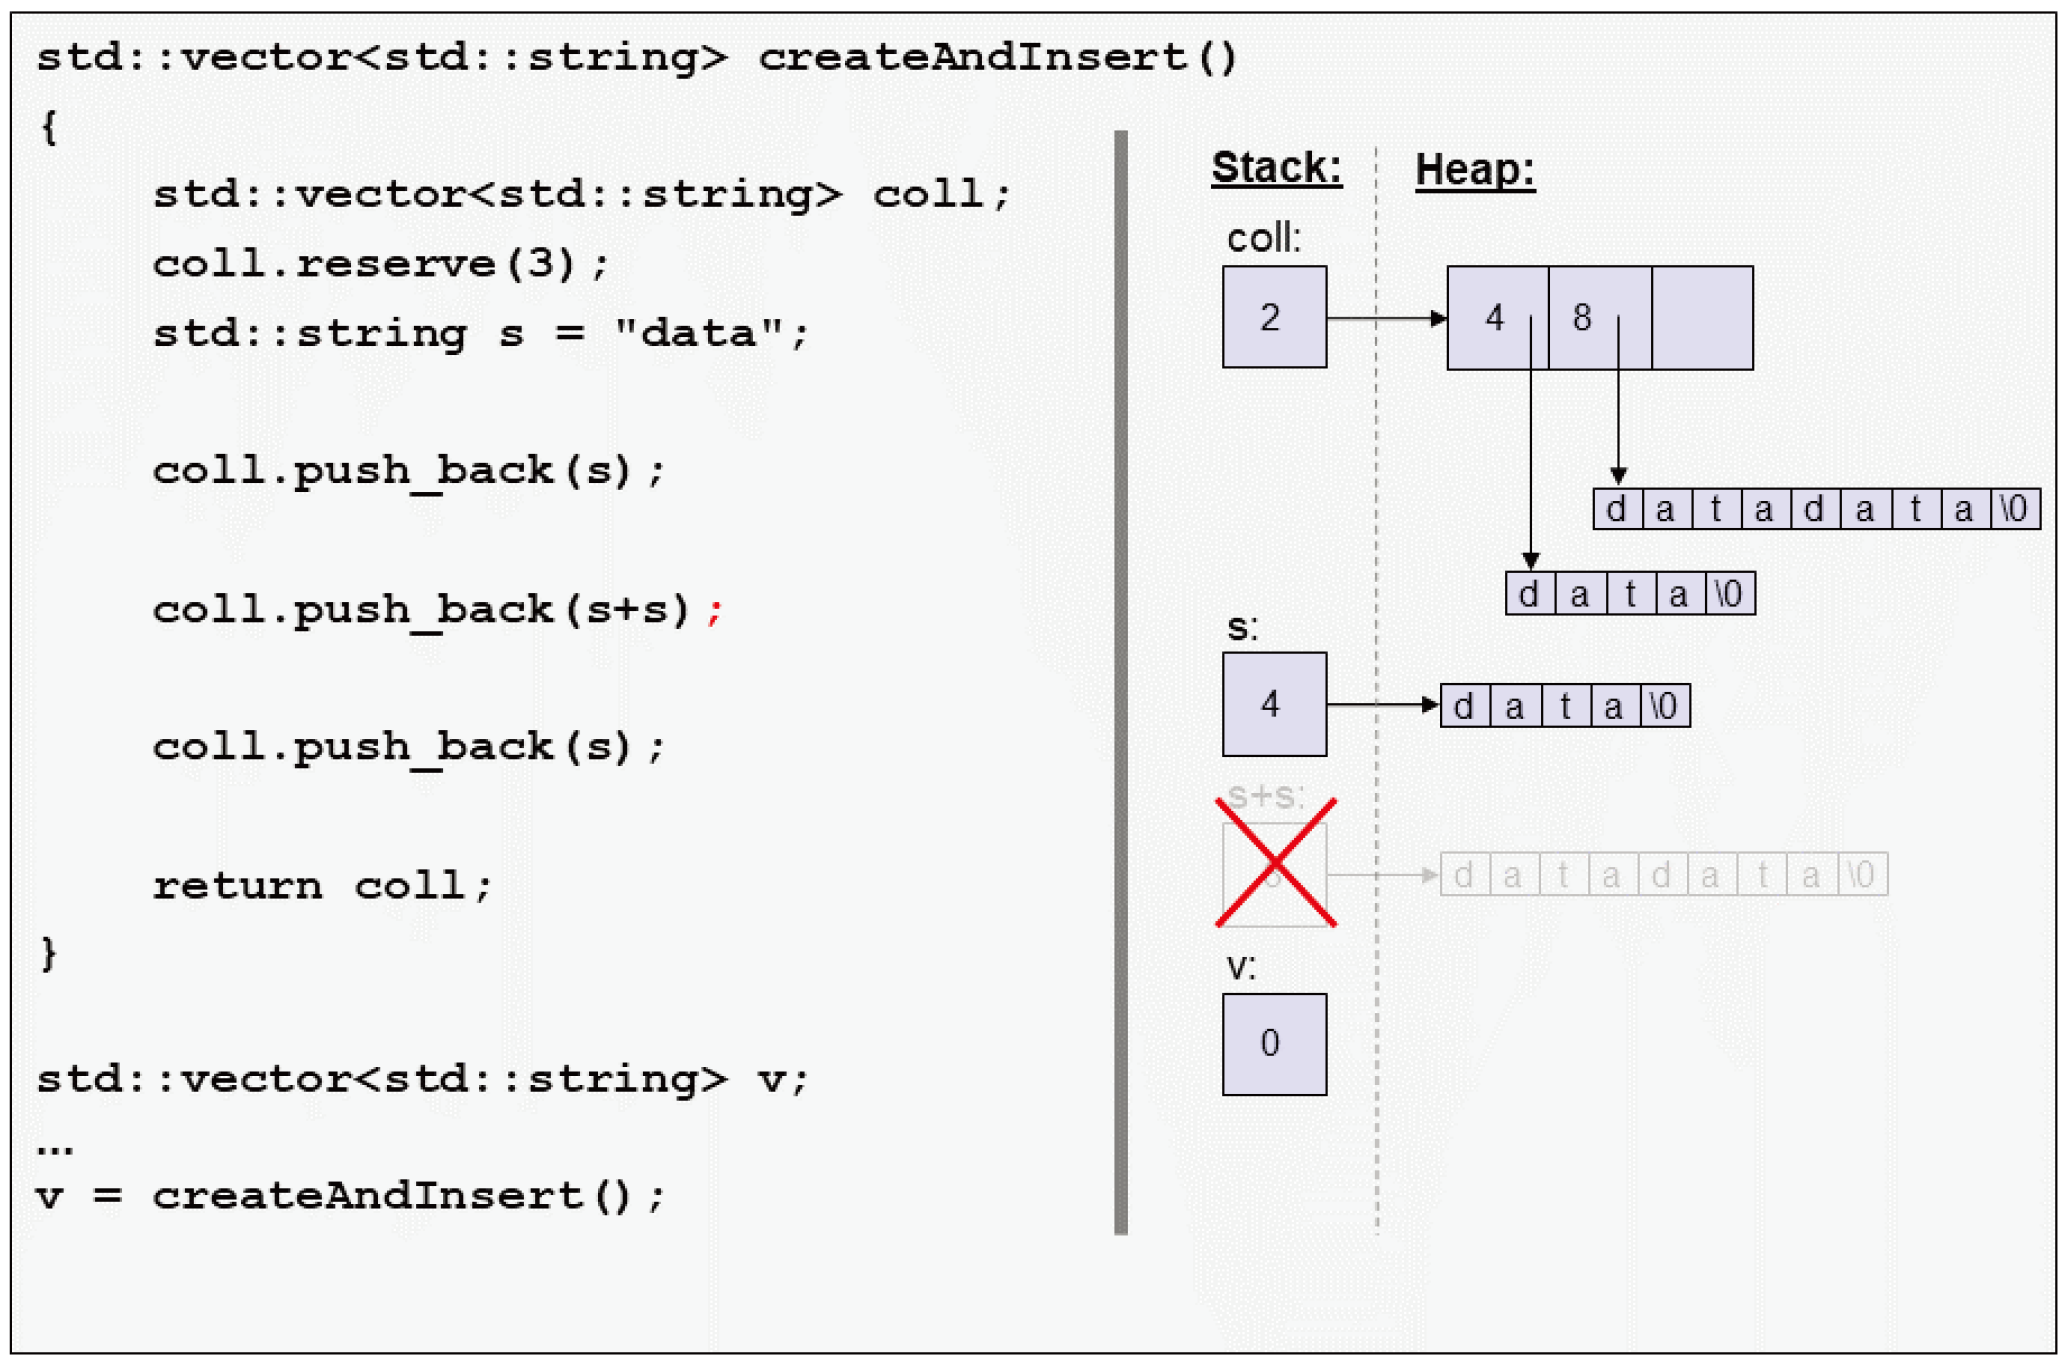
\includegraphics[width=1.0\textwidth]{content/1/chapter1/images/5}
		\end{center}
		这时我们第一次生成代码执行不大合适的地方:创建临时字符串的副本后销毁临时字符串。其实,可以不必分配和释放内存,直接使用原始的临时字符串对象。
	\end{enumerate}
	\item 下一行中,我们再将\textit{s}插入\textit{coll}中:\par
	\textbf{\textit{coll.push\_back(s);}}\par
	\textit{coll}继续拷贝\textit{s}:\par
	\begin{center}
		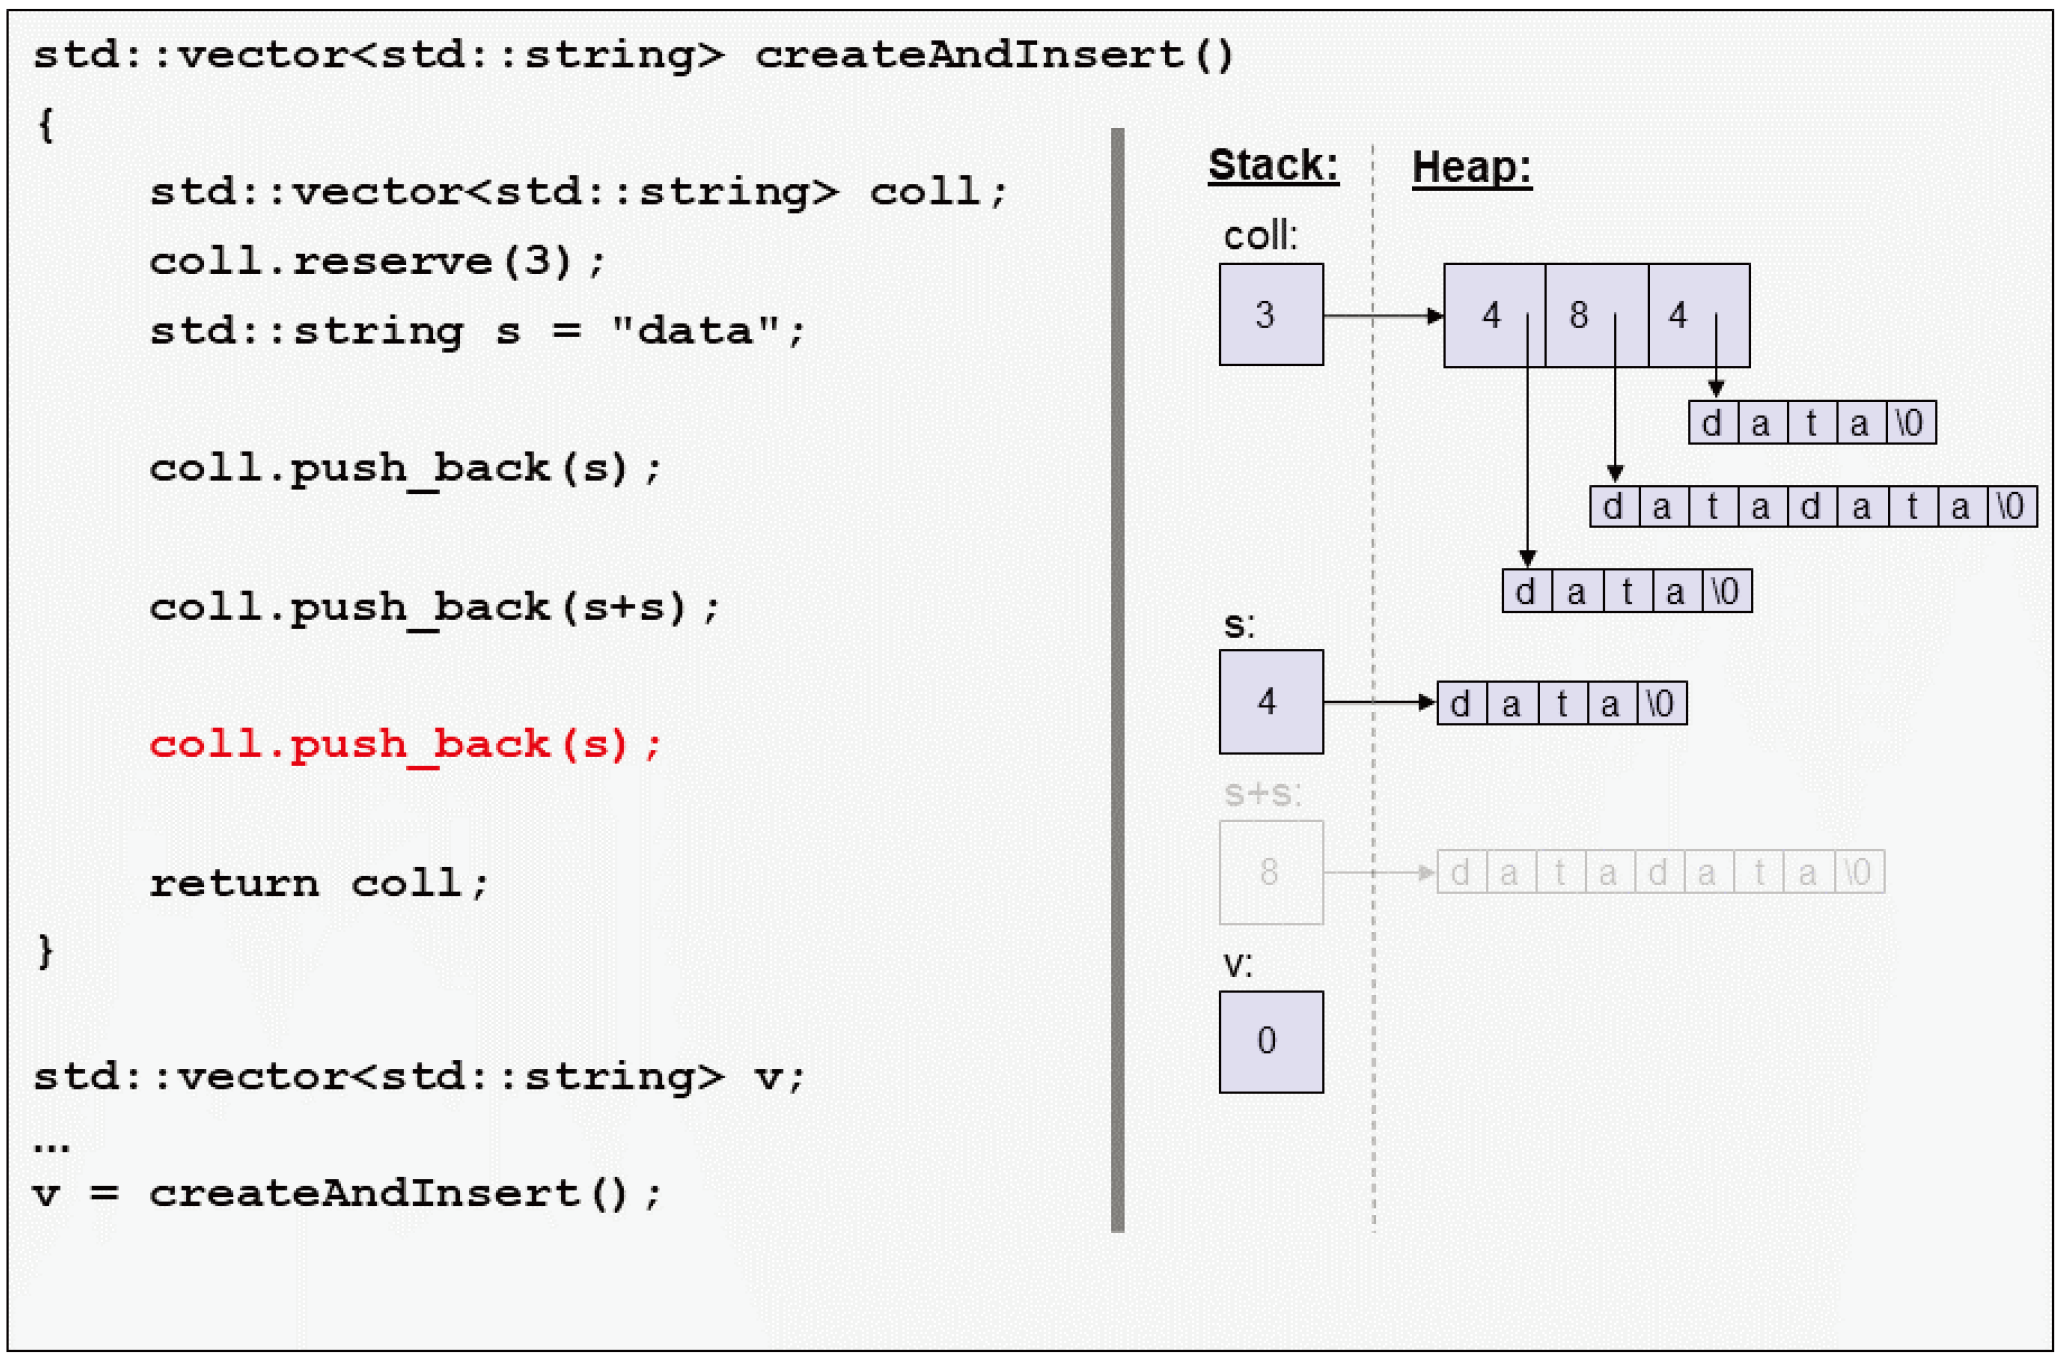
\includegraphics[width=1.0\textwidth]{content/1/chapter1/images/6}
	\end{center}
	这也是需要优化:一些优化技巧可以使用\textit{s}作为vector的新元素。
	\item 在\textit{createAndInsert()}的末尾,使用\textit{return}:\par
	\begin{lstlisting}[caption={}]
		return coll;
	}
	\end{lstlisting}
	程序的行为变得有点复杂。按值返回(返回类型不是引用)的应该是\textit{coll}的副本。创建副本意味着必须创建整个vector,及其所有元素的副本。因此,必须为vector中的元素数组分配堆内存,并为每个字符串分配用于保存其值的值分配堆内存。这样,我们需要分配4次内存。\par
	由于\textit{coll}被销毁,编译器可以执行命名返回值优化(NRVO)。这意味着编译器可以生成代码,使\textit{coll}只是用作返回值。\par
	可以使用这种优化,不过这可能会改变程序的行为。如果在vector或string对象的复制构造函数中有print语句,则会不看print语句的再次输出,这意味着这种优化改变了程序的功能行为。然而,这是可以的,因为在C++标准中允许这种优化,即使它有副作用。任何人都不应该知道这里有一个副本,是否执行命名返回值优化仅取决于编译器。\par
	假设我们进行了命名返回值优化,在\textit{return}语句的末尾,\textit{coll}现在成为返回值,并调用\textit{s}的析构函数,释放声明\textit{s}时分配的内存:\par
	\begin{center}
		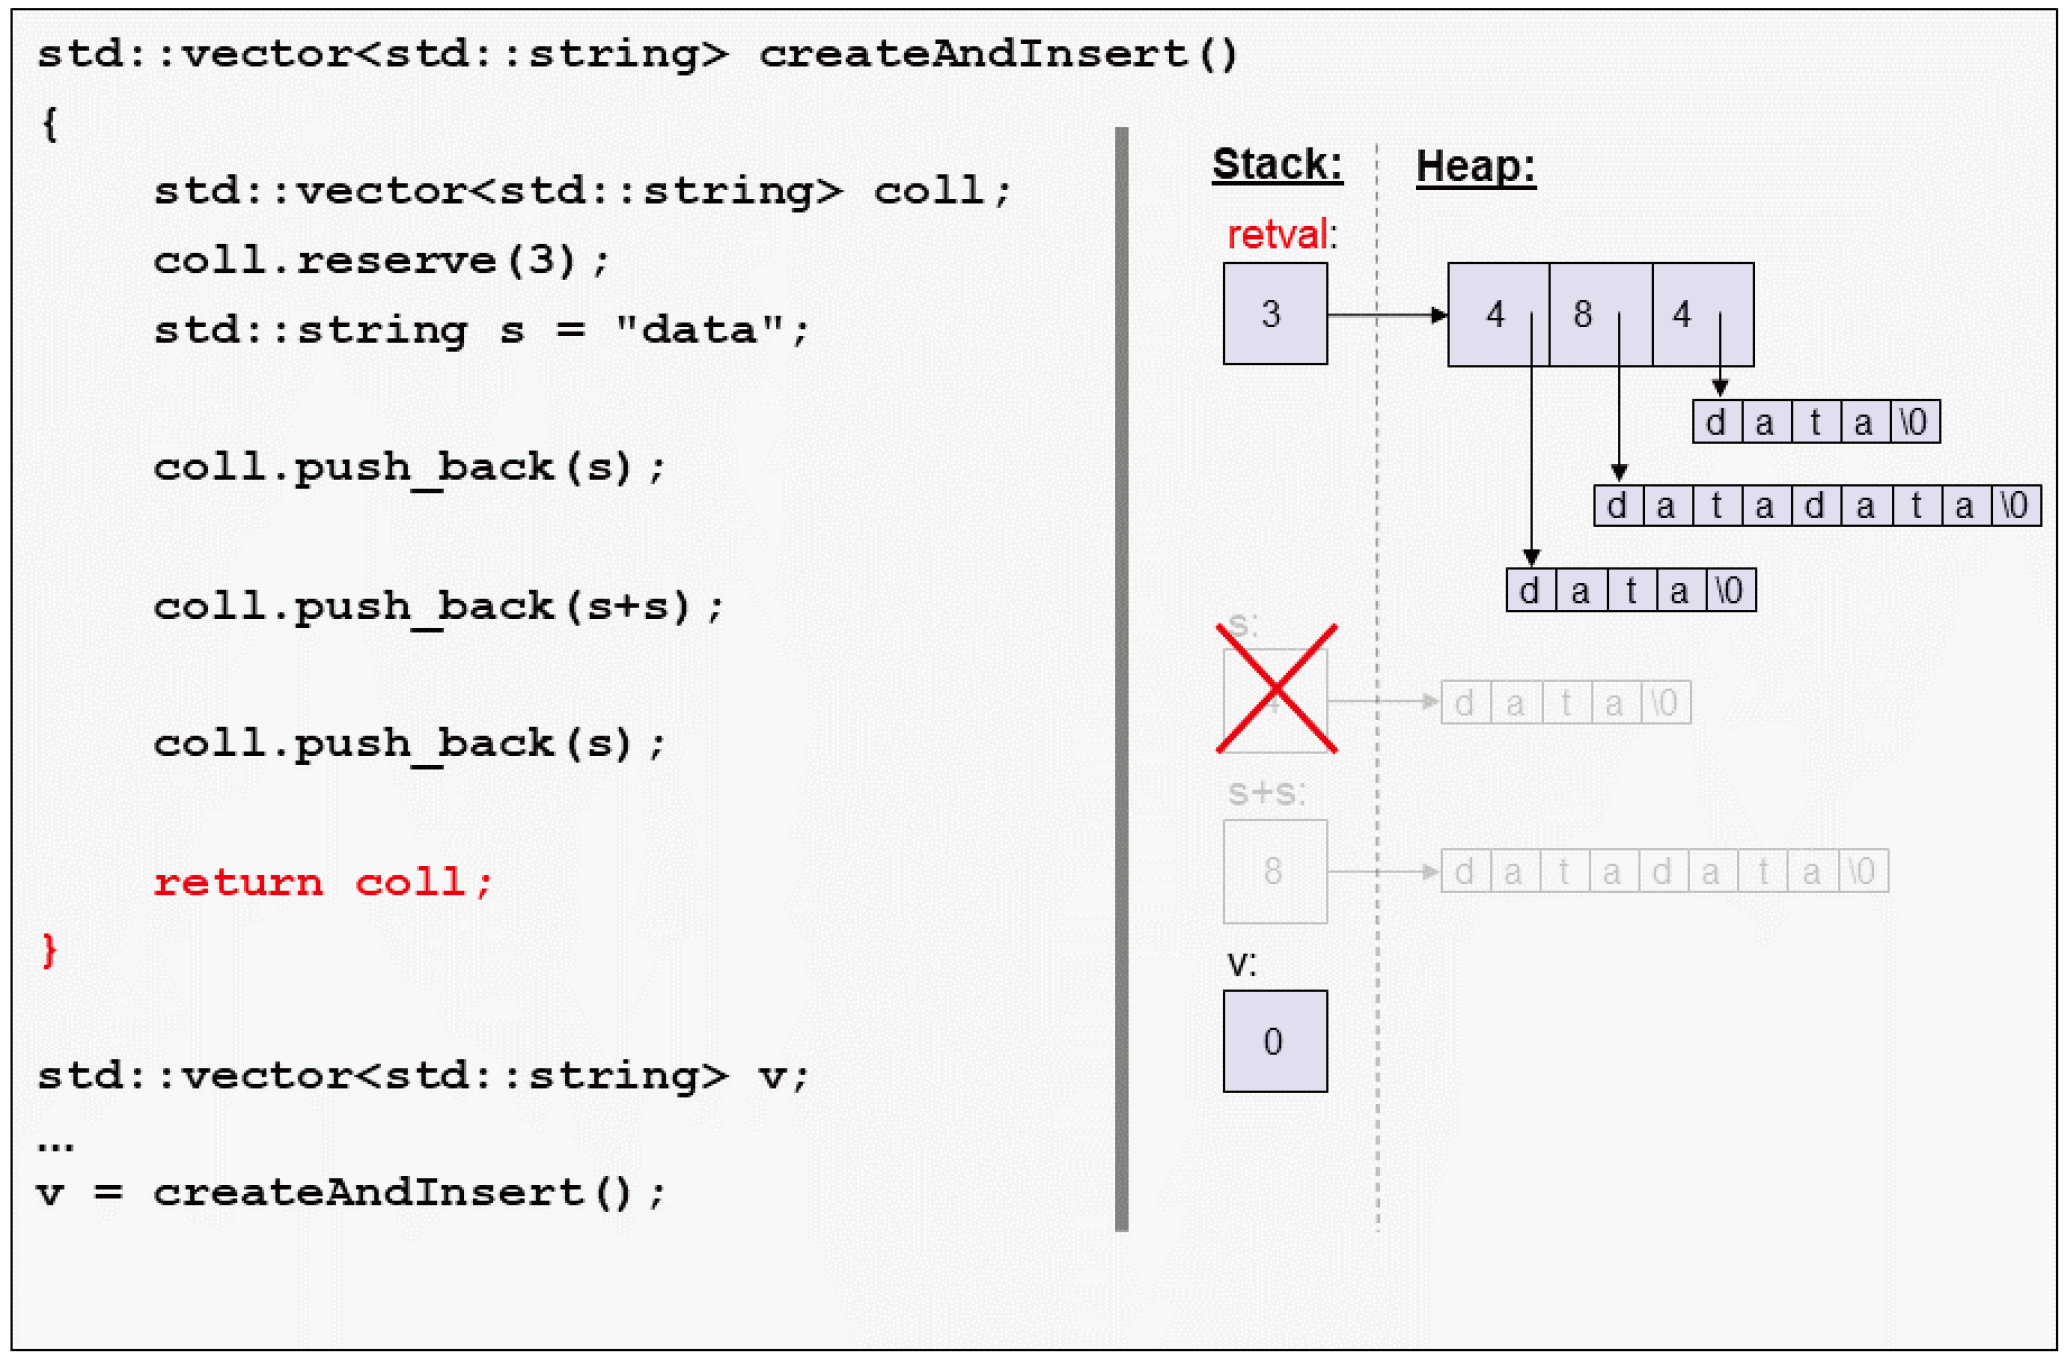
\includegraphics[width=1.0\textwidth]{content/1/chapter1/images/7}
	\end{center}
	\item 最后,将返回值赋给\textit{v}:\par
	\textbf{\textit{v = createAndInsert();}}\par
	这里可以改进的行为:通常的赋值操作符的目标是赋予\textit{v}与赋值源的值相同的值。一般来说,任何值都不应该被修改,并且应该独立于赋值的对象。因此,赋值操作符将创建了一个返回值的副本:\par
	\begin{center}
		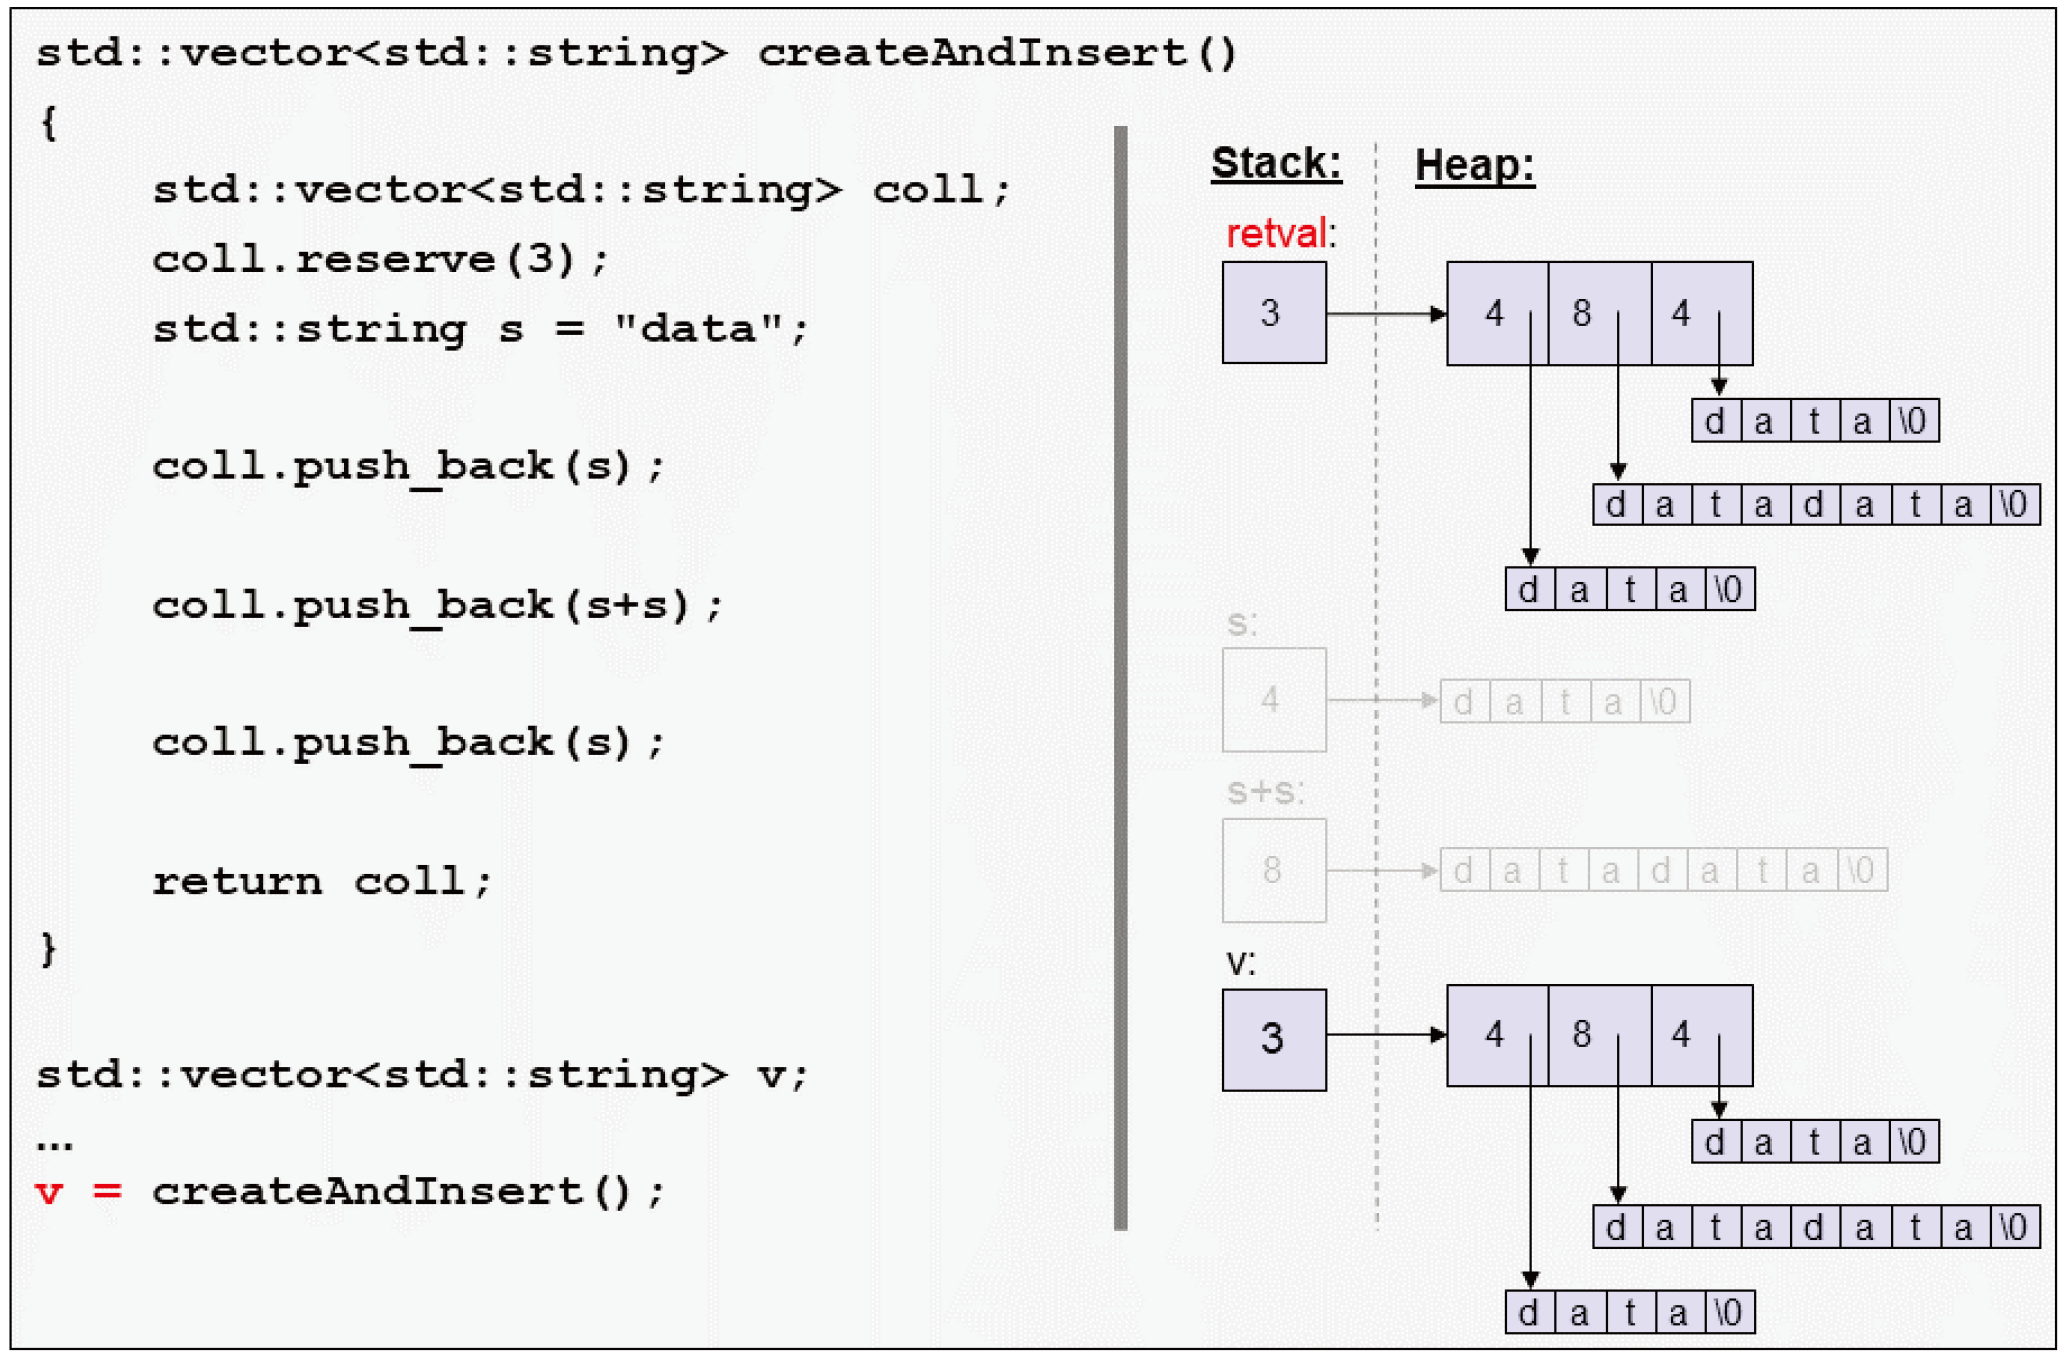
\includegraphics[width=1.0\textwidth]{content/1/chapter1/images/8}
	\end{center}
	之后,我们就不再需要临时返回值了,可以销毁它:\par
	\begin{center}
		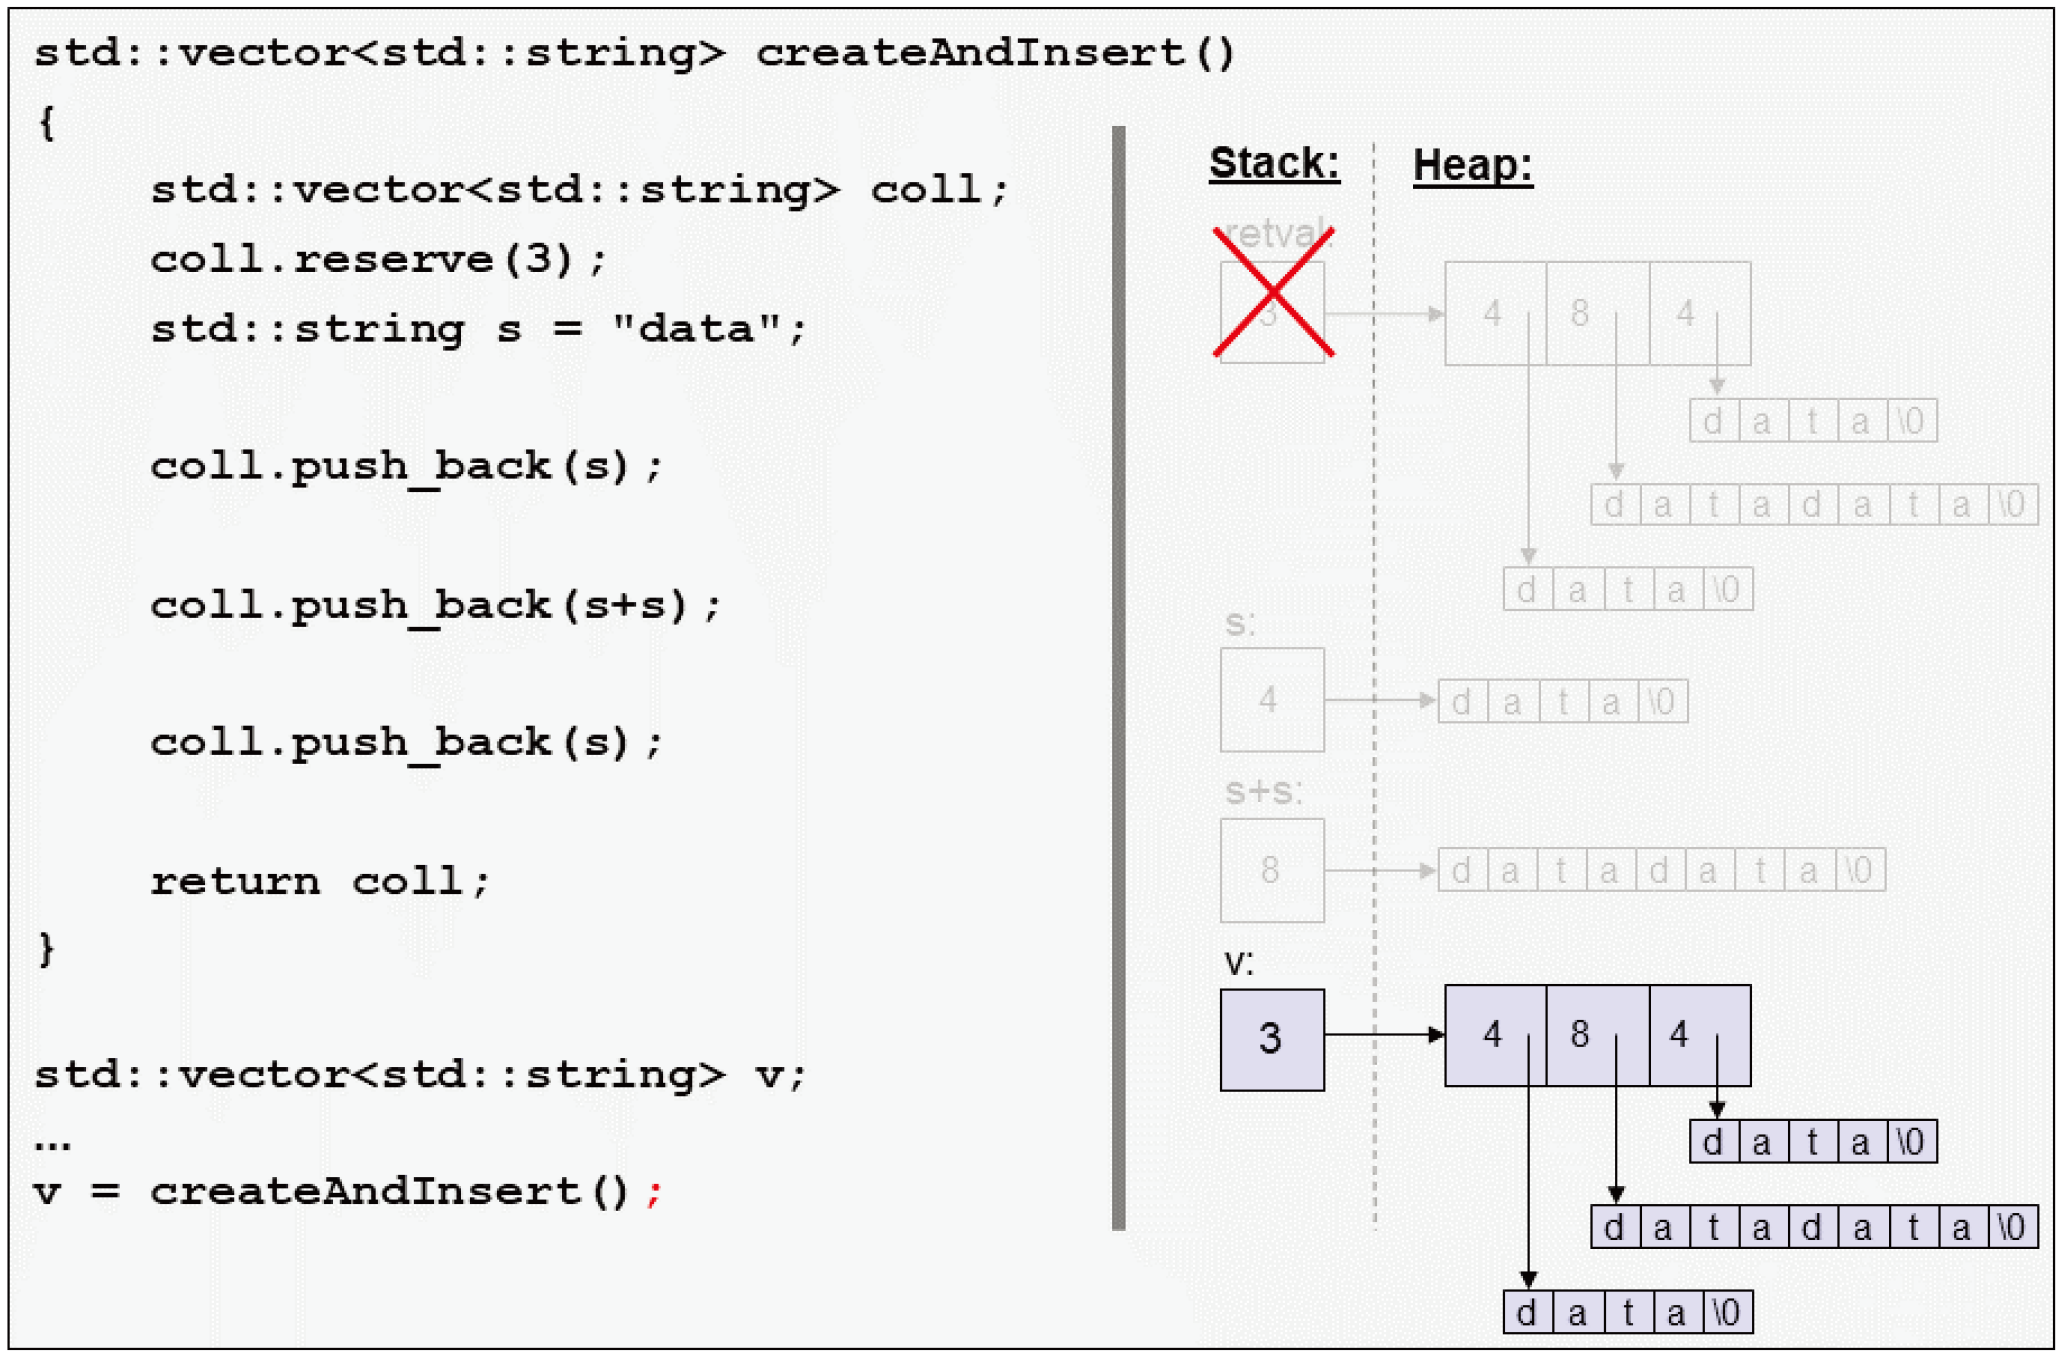
\includegraphics[width=1.0\textwidth]{content/1/chapter1/images/9}
	\end{center}
	我们创建了一个临时对象的副本,然后立即销毁该副本的源,再次分配和释放内存。这次适用于四个分配,一个分配给vector,其余分配给每个string元素。
\end{itemize}

对于\textit{main()}中赋值后的状态,分配了10次内存,释放了6次。不必要的内存分配由以下原因引起:\par

\begin{itemize}
	\item 将临时对象插入容器
	\item 将对象插入到不再需要该值的容器中
	\item 将一个临时vector的值赋于其他对象
\end{itemize}

我们可以或多或少地避免这些性能损失。我们可以这样做:\par

\begin{itemize}
	\item 将vector作为out参数传递:\par
	\textit{\textbf{createAndInsert(v); {\color{mygreen}{// let the function fill vector v}}}}
	\item 使用swap():\par
	\textit{\textbf{createAndInsert().swap(v);}}
\end{itemize}

但是,得到的代码看起来更难看懂(除非您在复杂的代码中看到一些美),而且在插入临时对象时没有真正的解决问题。\par

自C++11起,我们有了另一个选择:编译并运行支持移动语义的程序。\par

\hspace*{\fill} \par %插入空行
\textbf{使用C++11的例子(使用移动语义)}

现在让我们用一个支持移动语义的现代C++编译器(C++11或更高版本)重新编译这个程序:\par

{\color{red}{basics/motiv11.cpp}}

\begin{lstlisting}[caption={}]
#include <string>
#include <vector>

std::vector<std::string> createAndInsert()
{
	std::vector<std::string> coll; // create vector of strings
	coll.reserve(3); // reserve memory for 3 elements
	std::string s = "data"; // create string object
	
	coll.push_back(s); // insert string object
	coll.push_back(s+s); // insert temporary string
	coll.push_back(std::move(s)); // insert string (we no longer need the value of s)
	
	return coll; // return vector of strings
}

int main()
{
	std::vector<std::string> v; // create empty vector of strings
	...
	v = createAndInsert(); // assign returned vector of strings
	...
}
\end{lstlisting}

这里有一个小修改:将最后一个元素插入\textit{coll}时,添加了\textit{std::move()}的调用,我们将在讨论这个语句时聊聊这个更改。其他都和之前一样。\par

让我们再次通过检查堆栈和堆来了解程序的各个步骤。\par

\begin{itemize}
	\item 首先,在\textit{main()}中创建空vector \textit{v},包含0个元素:\par
	\textit{\textbf{std::vector<std::string> v;}}
	\item 之后,调用:\par
	\textit{\textbf{v = createAndInsert();}}\par
	在堆栈上创建另一个空vector \textit{coll},并保留三个元素未初始化的内存:\par
	\textit{\textbf{std::vector<std::string> coll;}}\par
	\textit{\textbf{coll.reserve(3);}}\par
	\item 然后,我们创建用“data”初始化的字符串\textit{s},并再次将其插入\textit{coll}中:\par
	\textit{\textbf{std::string s = "data";}}
	\textit{\textbf{coll.push\_back(s);}}
	目前为止,还没有什么需要优化的,程序状态与C++03相同:\par
	\begin{center}
		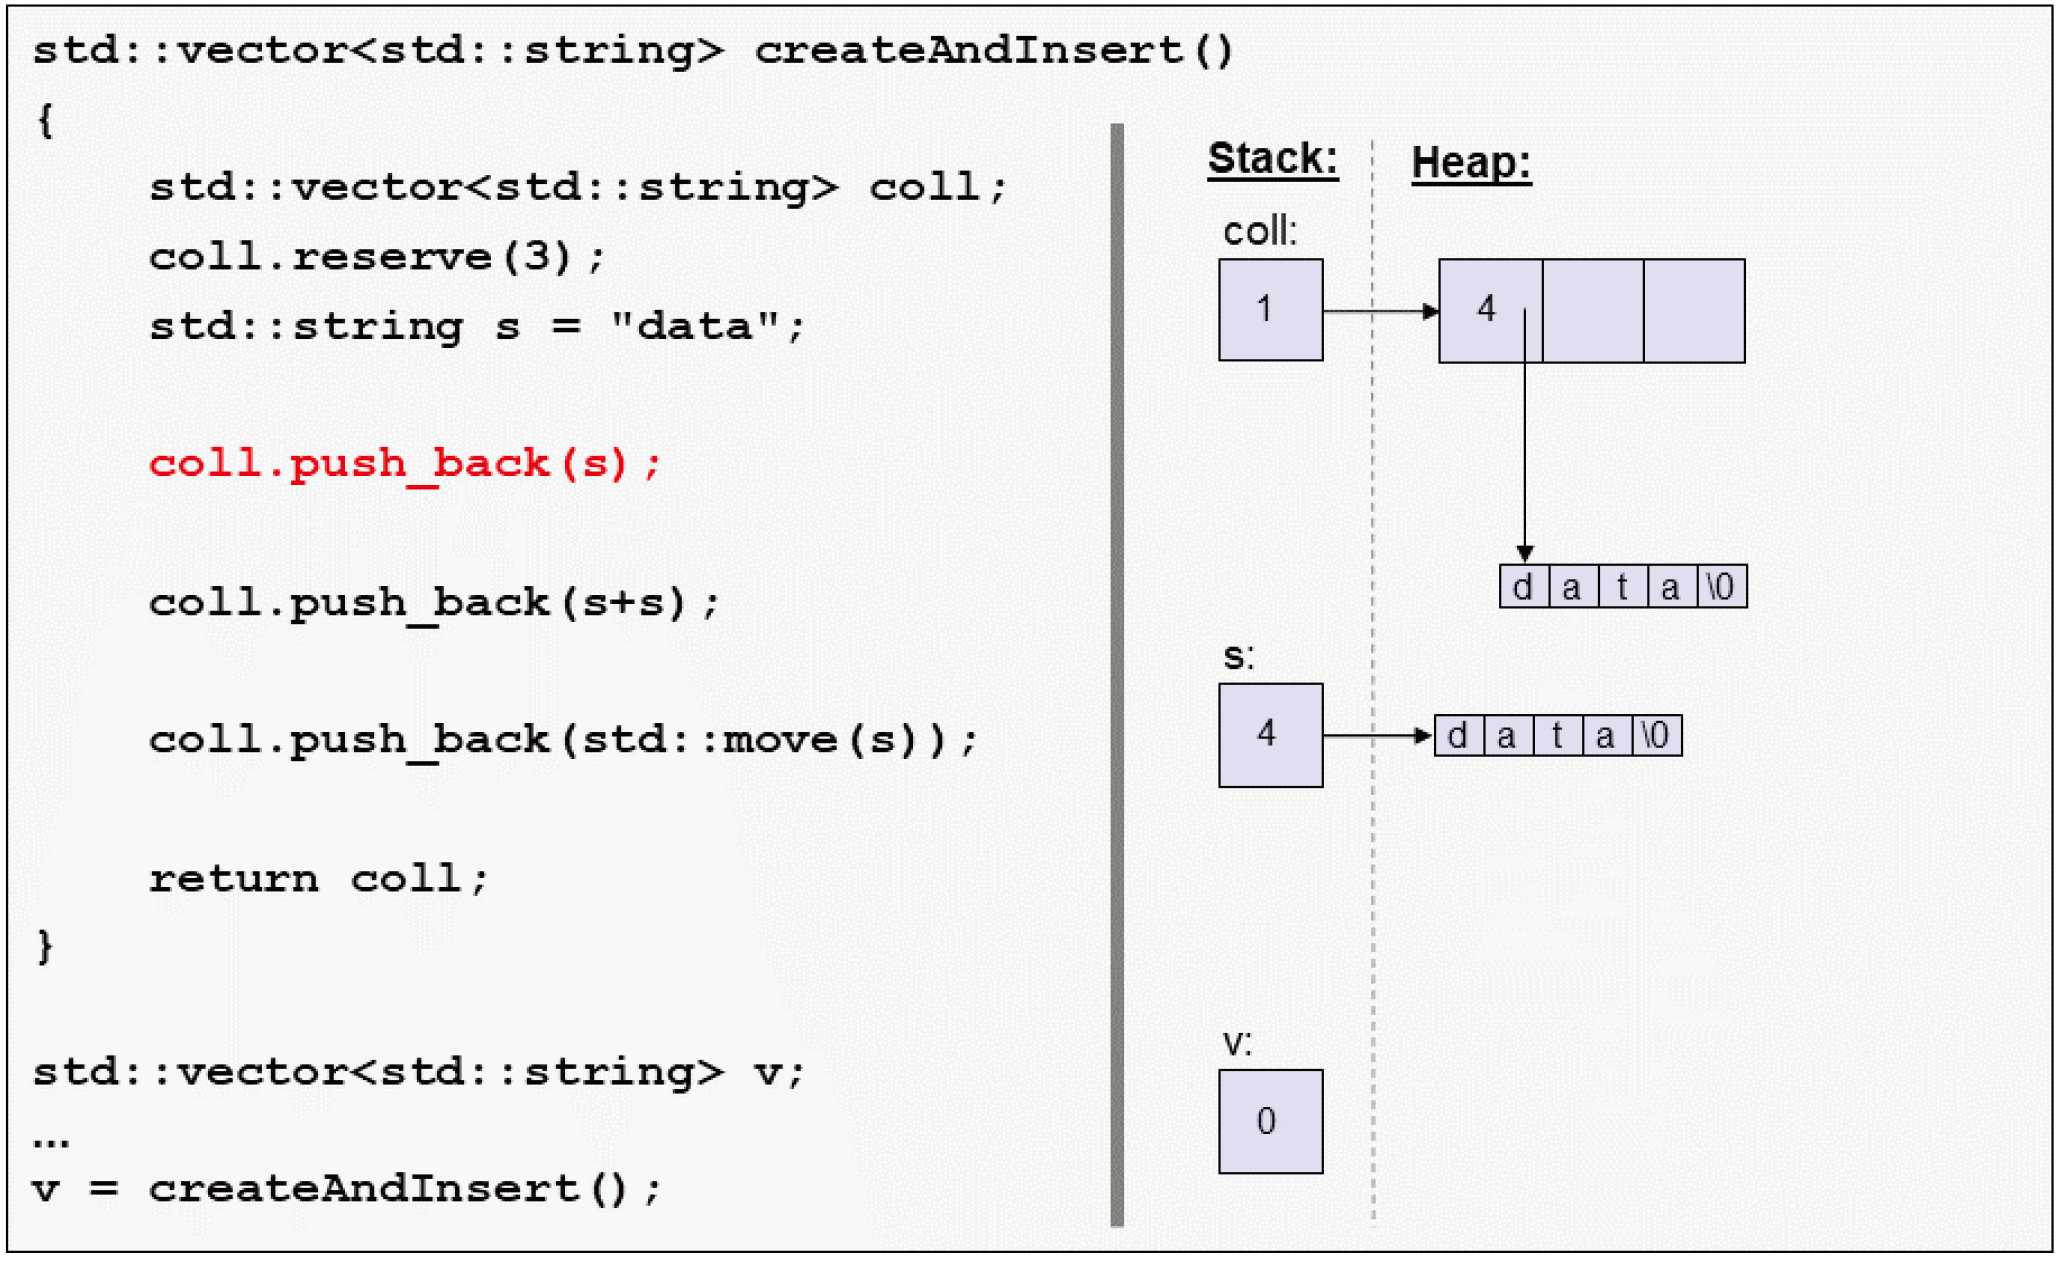
\includegraphics[width=1.0\textwidth]{content/1/chapter1/images/10}
	\end{center}
	我们有两个vector,\textit{v}和\textit{coll},还有两个字符串,\textit{s}和它的副本,也就是\textit{coll}的第一个元素。它们都是独立的对象,有自己的内存。\par
	\item 首先,看看创建一个新的临时字符串并将其插入vector中的语句:\par
	\textit{\textbf{coll.push\_back(s+s);}}\par
	同样,该语句分三个步骤执行:\par
	\begin{enumerate}
		\item 创建临时字符串\textit{s+s}:\par
		\begin{center}
			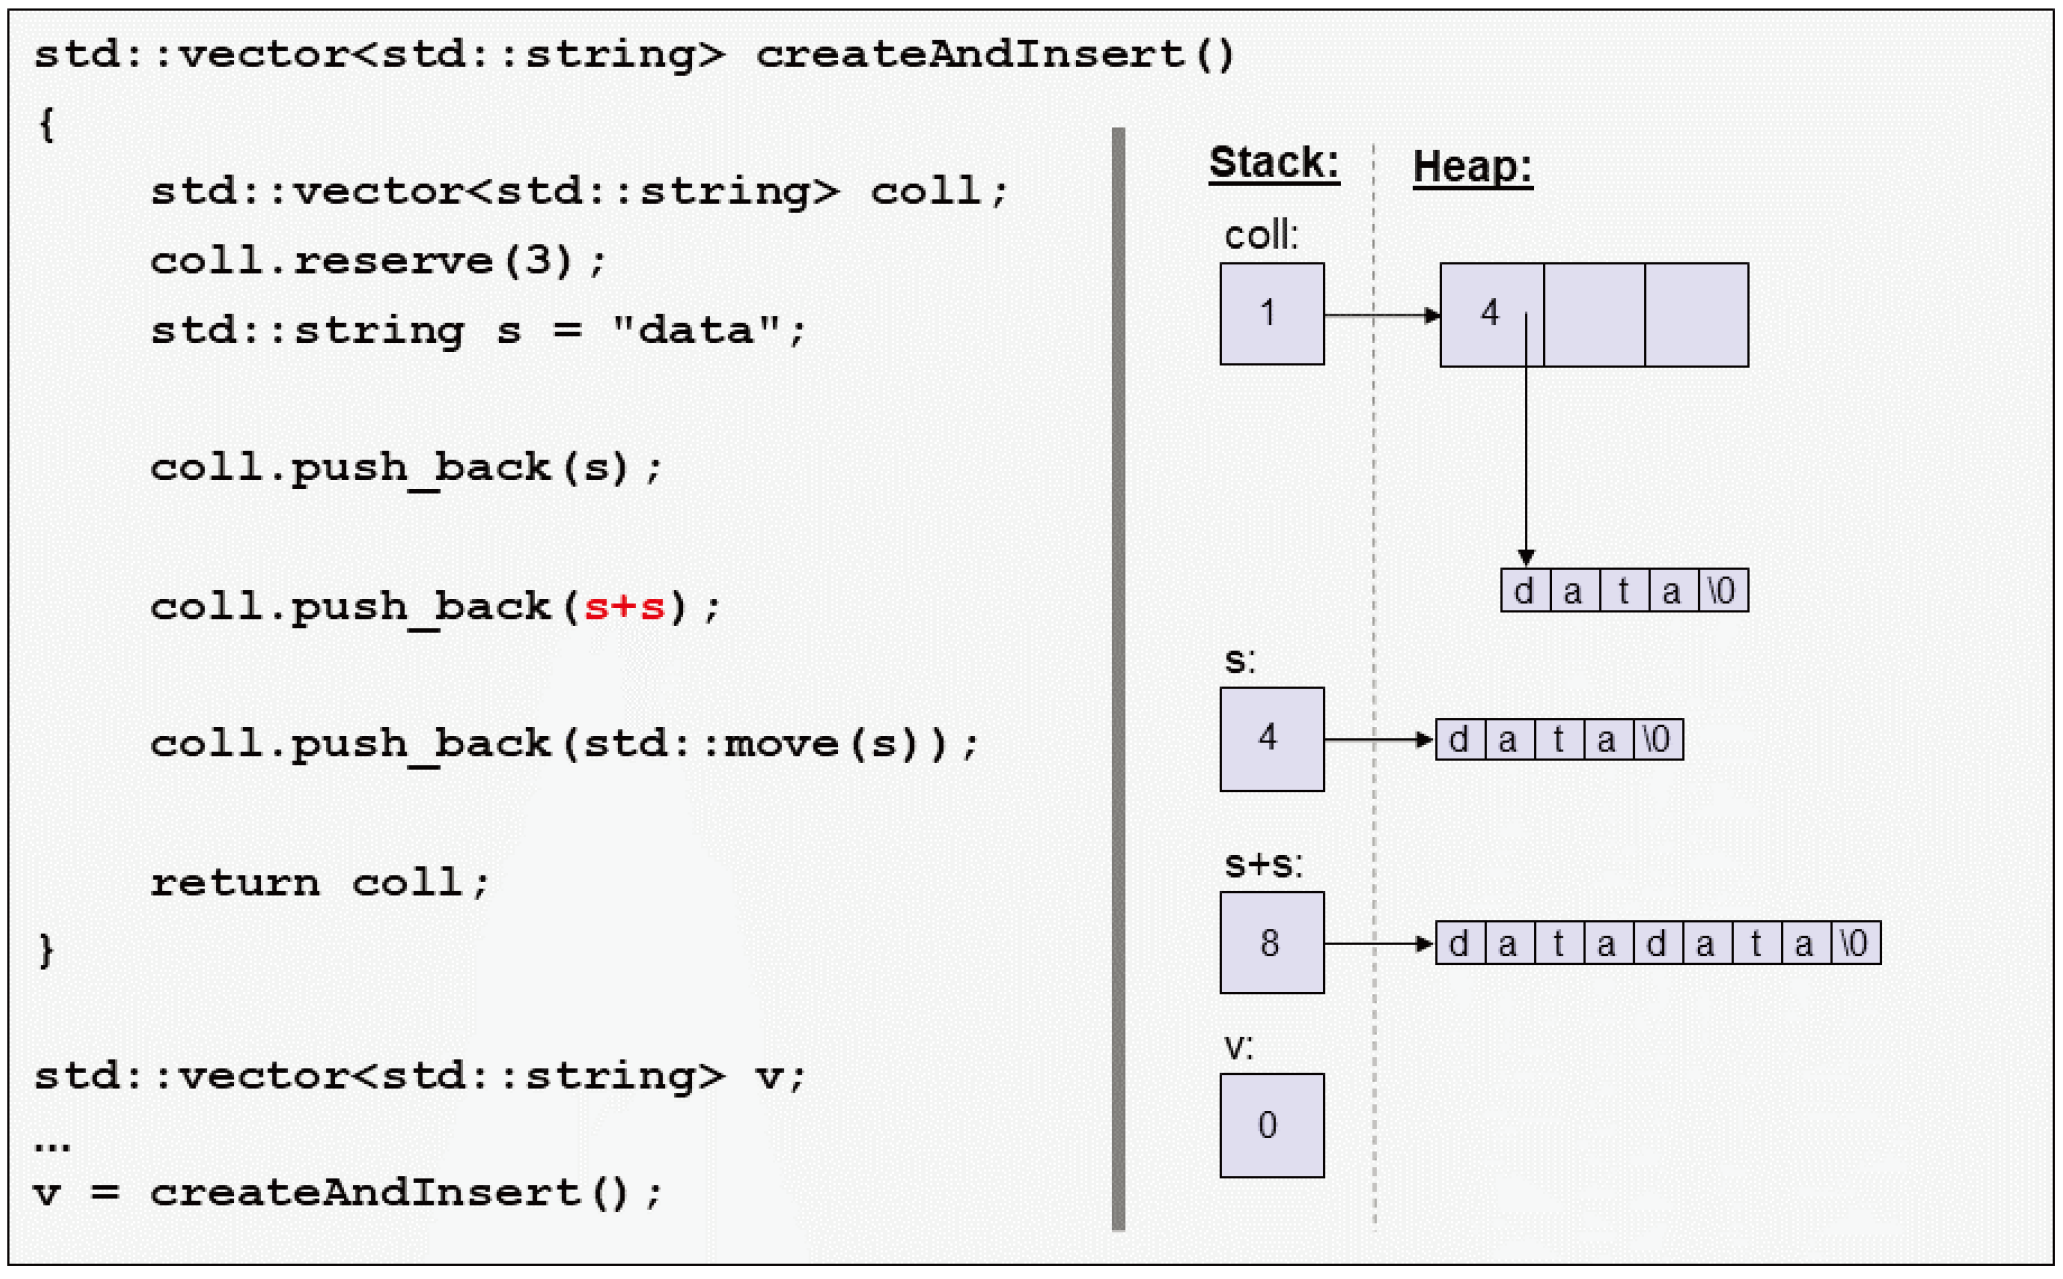
\includegraphics[width=1.0\textwidth]{content/1/chapter1/images/11}
		\end{center}
		\item 将这个临时字符串插入到\textit{coll}中。然而,这里发生了一些不同的事情:我们从\textit{s+s}中窃取了内存,并将其移动到\textit{coll}的新元素中。\par
		\begin{center}
			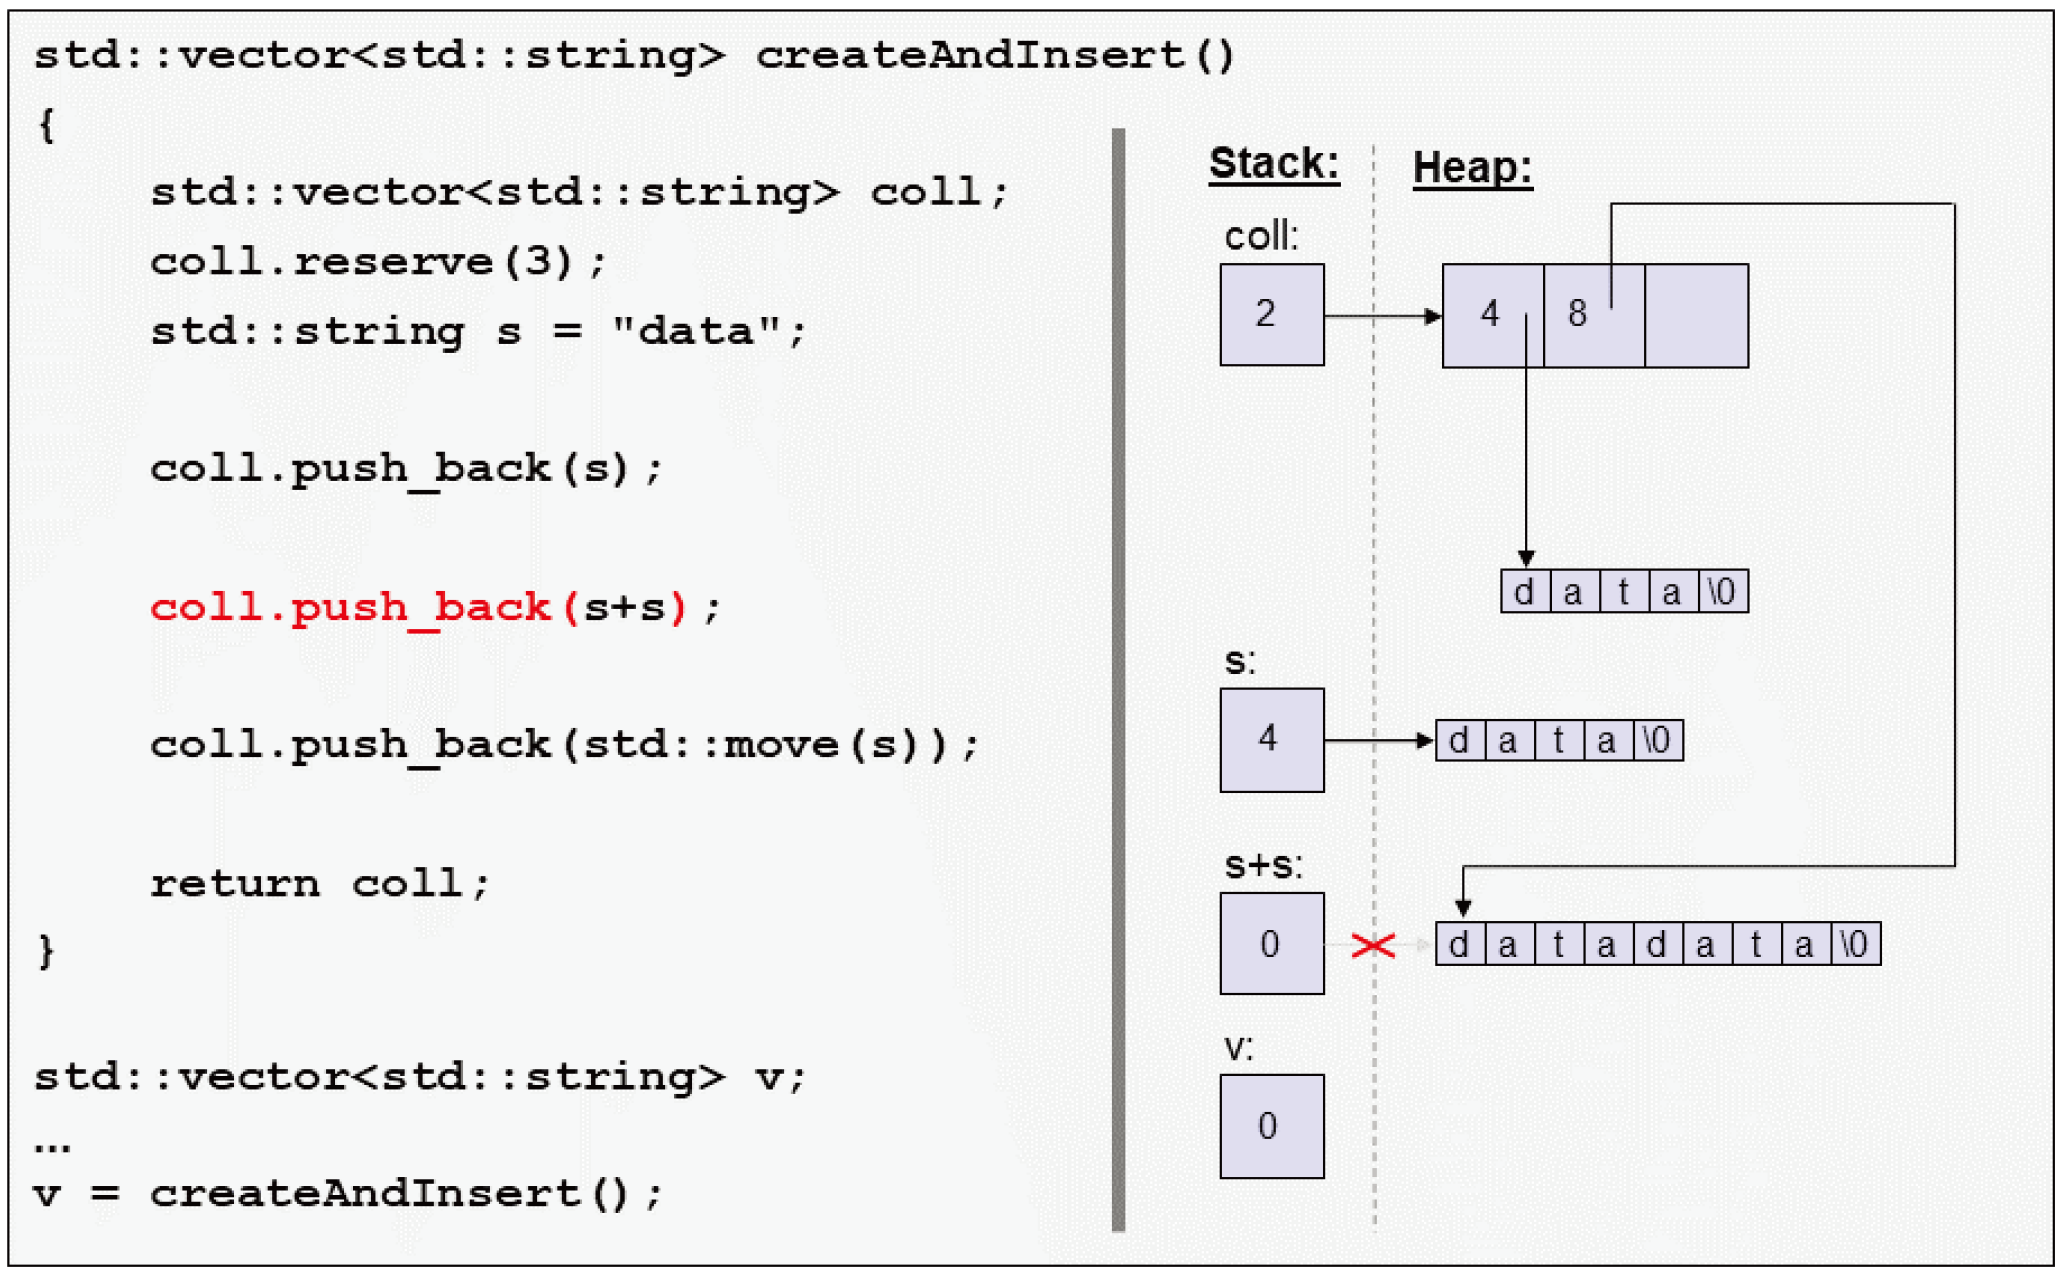
\includegraphics[width=1.0\textwidth]{content/1/chapter1/images/12}
		\end{center}
		从c++ 11开始,我们可以获取不再需要的值。因为编译器知道在执行push\_back()调用之后,临时对象\textit{s+s}将被销毁。因此,调用的是push\_back()的另一个实现,其是对不再需要值的字符串进行复制的优化:我们复制了大小和指向内存的指针,而不是创建拷贝。然而,这种浅复制是不够的;我们还修改了临时对象\textit{s+s},将其大小设置为0,并将nullptr赋值为新值。其实,s+s被修改了,以便呈现空字符串的状态。重要的是,它不再拥有自己的内存。
		\item 在语句的结尾,临时字符串\textit{s+s}被销毁。但由于临时字符串不再是初始内存的所有者,析构函数不会释放该内存。\par
		\begin{center}
			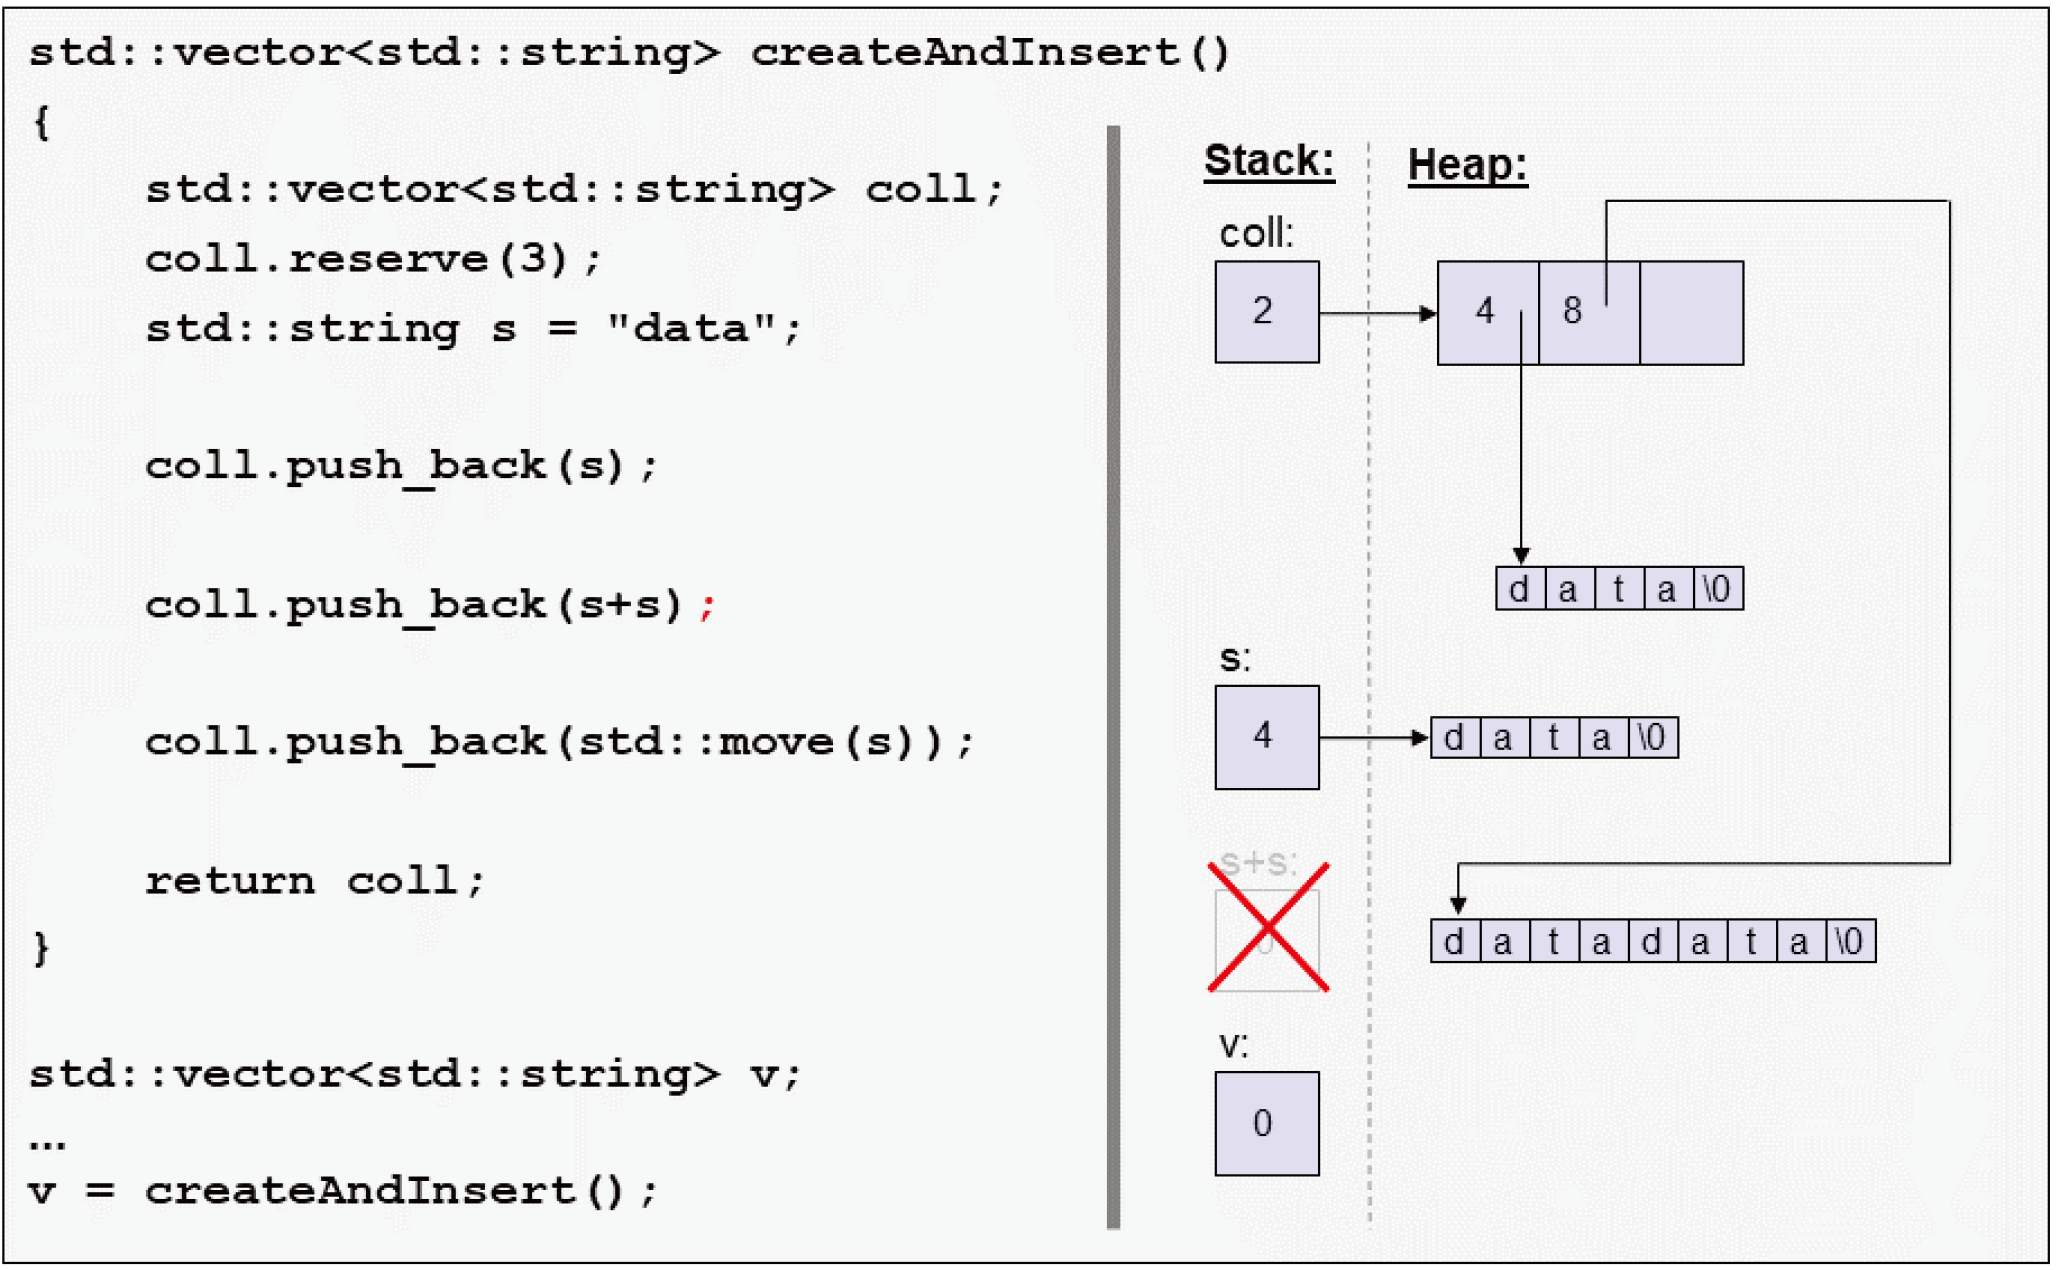
\includegraphics[width=1.0\textwidth]{content/1/chapter1/images/13}
		\end{center}
		我们优化了复制过程,将\textit{s+s}的内存所有权转移到它在vector中的副本。\par
		这一切都是通过编译器自动完成的,编译器可以对即将死亡的对象发出信号,我们可以使用新实现来复制一个从源端窃取值的字符串值。这不是一个技巧,这是一种语义上的移动,通过从底层技术上将值的内存从源字符串移动到它的副本来实现。\par
	\end{enumerate}
	\item 下一条语句是我们为C++11版本修改的语句。将\textit{s}插入到\textit{coll}中,但是通过对要插入的字符串\textit{s}调用\textit{std::move()},语句发生了改变:\par
	\textit{\textbf{coll.push\_back(std::move(s));}}\par
	如果没有\textit{std::move()},就会像第一次调用\textit{push\_back()}一样:vector会创建传递的字符串\textit{s}的副本。这次,我们用\textit{std::move()}标记了\textit{s},这在意味着明示“这里不再需要这个值”。因此,这里会使用另一个\textit{push\_back()}实现,它会在传递临时对象\textit{s+s}时使用。第三个元素通过将这个值的内存所有权,从\textit{s}转移到副本中,从而来窃取这个值:\par
	\begin{center}
		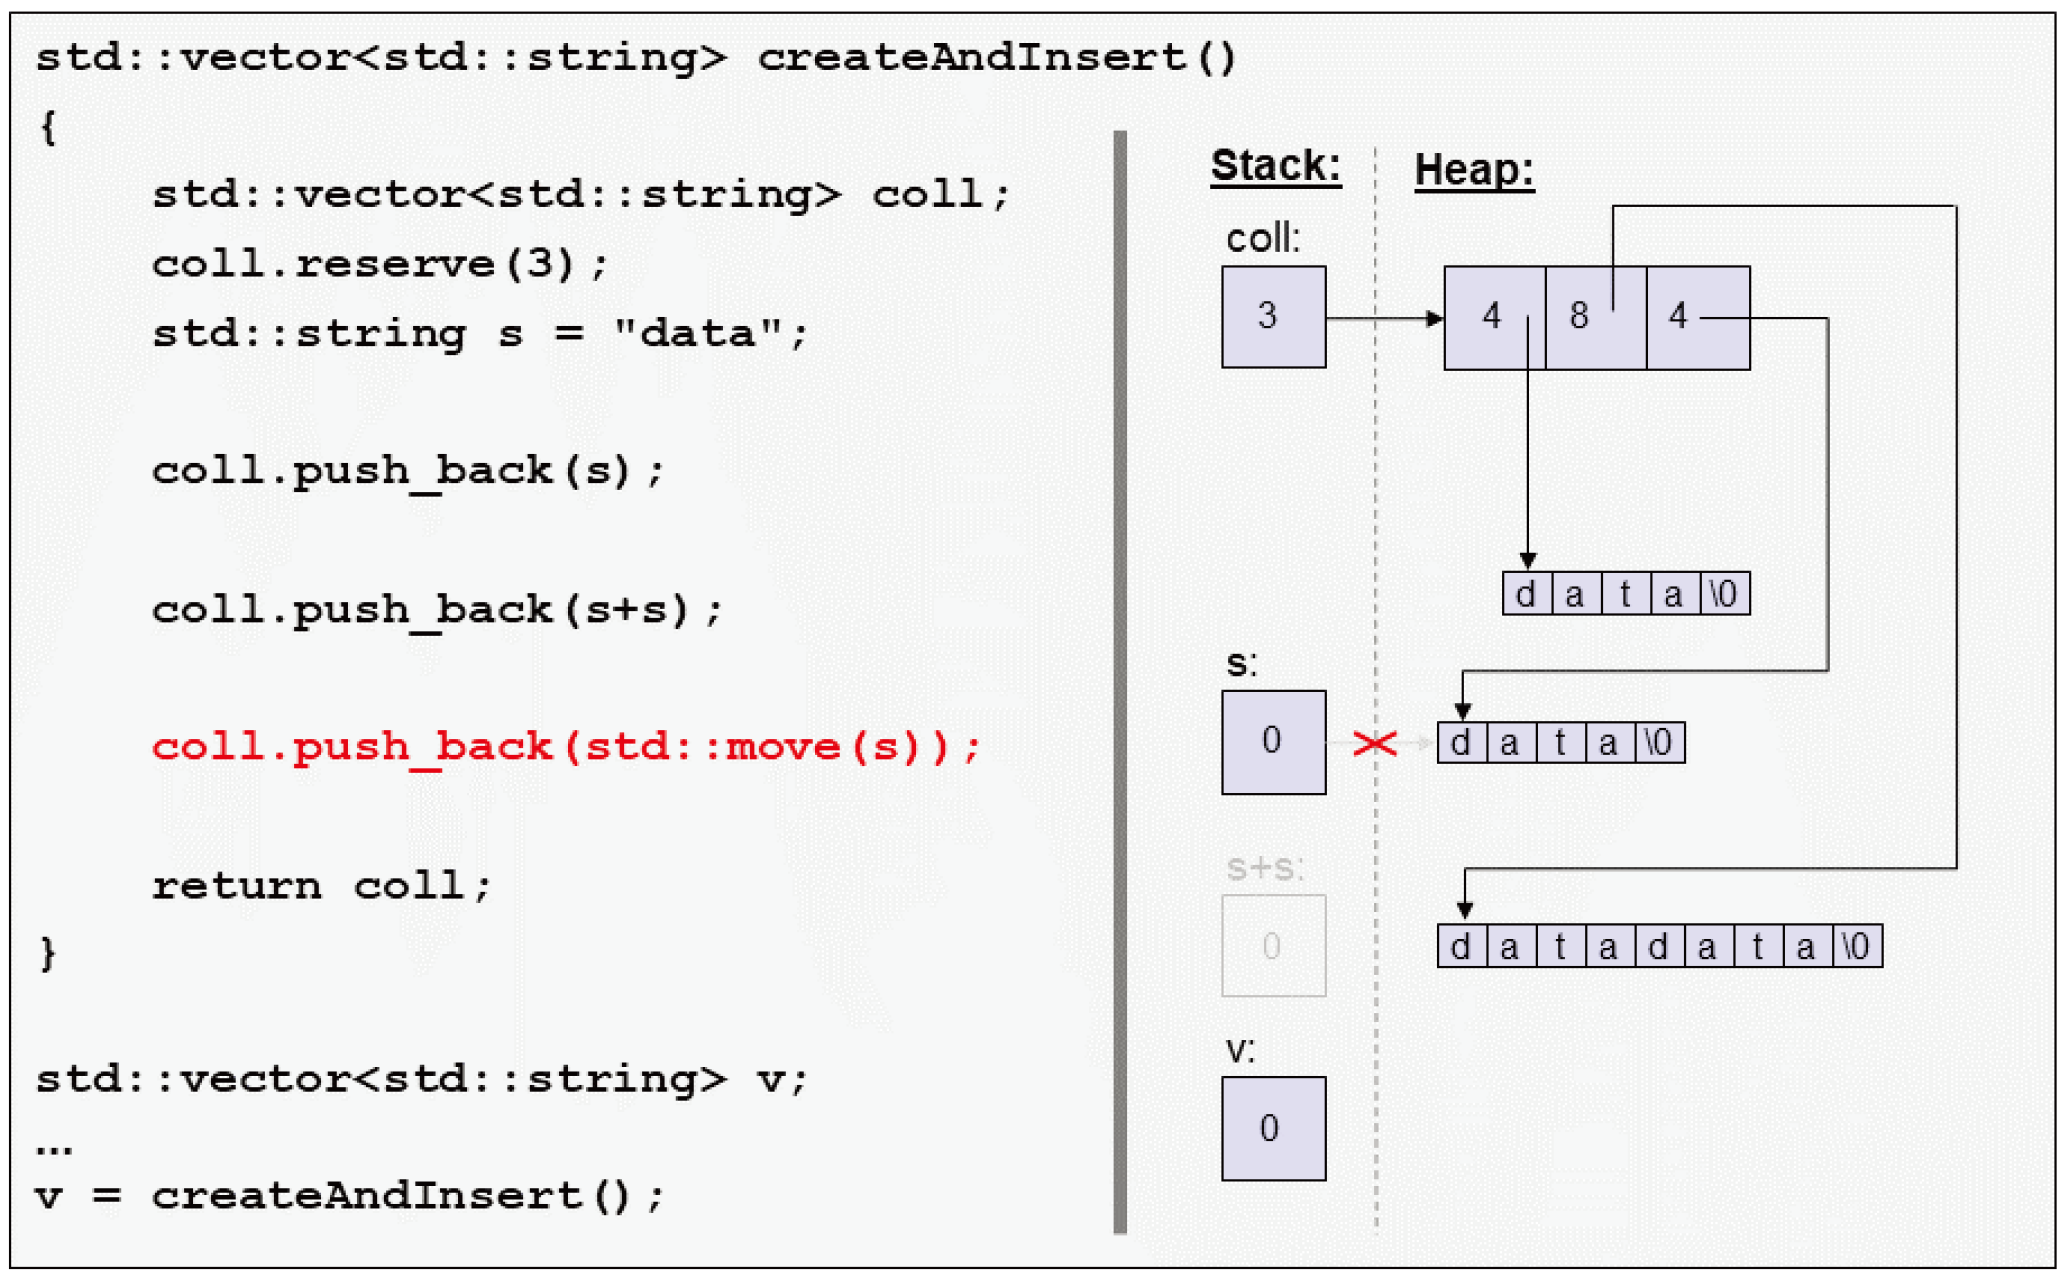
\includegraphics[width=1.0\textwidth]{content/1/chapter1/images/14}
	\end{center}
	关于移动语义,请注意以下两点:\par
	\begin{itemize}
		\item[-] \textit{std::move(s)}在这里只表示\textit{s}是可移动的。只是说,我不再需要这个值,它允许实现通过在复制值时进行一些优化(比如偷取内存)从而获益。调用者并不知道值是否进行了移动。
		\item[-] 然而,窃取值的优化必须确保源对象仍然处于有效状态。被移动的对象既不会部分销毁,也不会完全销毁。C++标准库为它的类型进行了规定:标记为\textit{std::move()}的对象执行操作后,该对象处于有效,但未定义的状态。\par
		以上,就是在这条语句执行完成后会发生的事\par
		\textit{\textbf{coll.push\_back(std::move(s));}}\par
		这里保证\textit{s}仍然是有效的字符串。这就像使用不知道传递了哪个值的字符串参数一样。\par
		注意,它也不能保证字符串要么有旧值,要么为空。它的值由运行时库实现者决定。通常,实现者可以对\textit{std::move()}操作的对象做任何事,只要保持对象的有效状态。保证的理由,稍后讨论。
	\end{itemize}
	
	\item createAndInsert()最后的return语句为:\par
	\begin{lstlisting}[caption={}]
		return coll;
	}
	\end{lstlisting}
	是否生成具有指定返回值优化的代码取决于编译器,\textit{coll}只是成为了返回值。但是,如果不使用这种优化,return语句仍然是从即将失效的源创建对象的情况。如果没有使用指定的返回值优化,仍然会使用移动语义,返回值会从\textit{coll}中窃取值。在最坏的情况下,必须从源文件复制成员的大小、容量和指向内存的指针(总共12或24个字节)到返回值中,并在源文件中为这些成员赋值。\par
	我们假设进行了返回值优化。在return语句中,\textit{coll}成为返回值,并调用\textit{s}的析构函数,不再需要释放任何内存,因为内存移到了\textit{coll}的第三个元素中:\par
	\begin{center}
		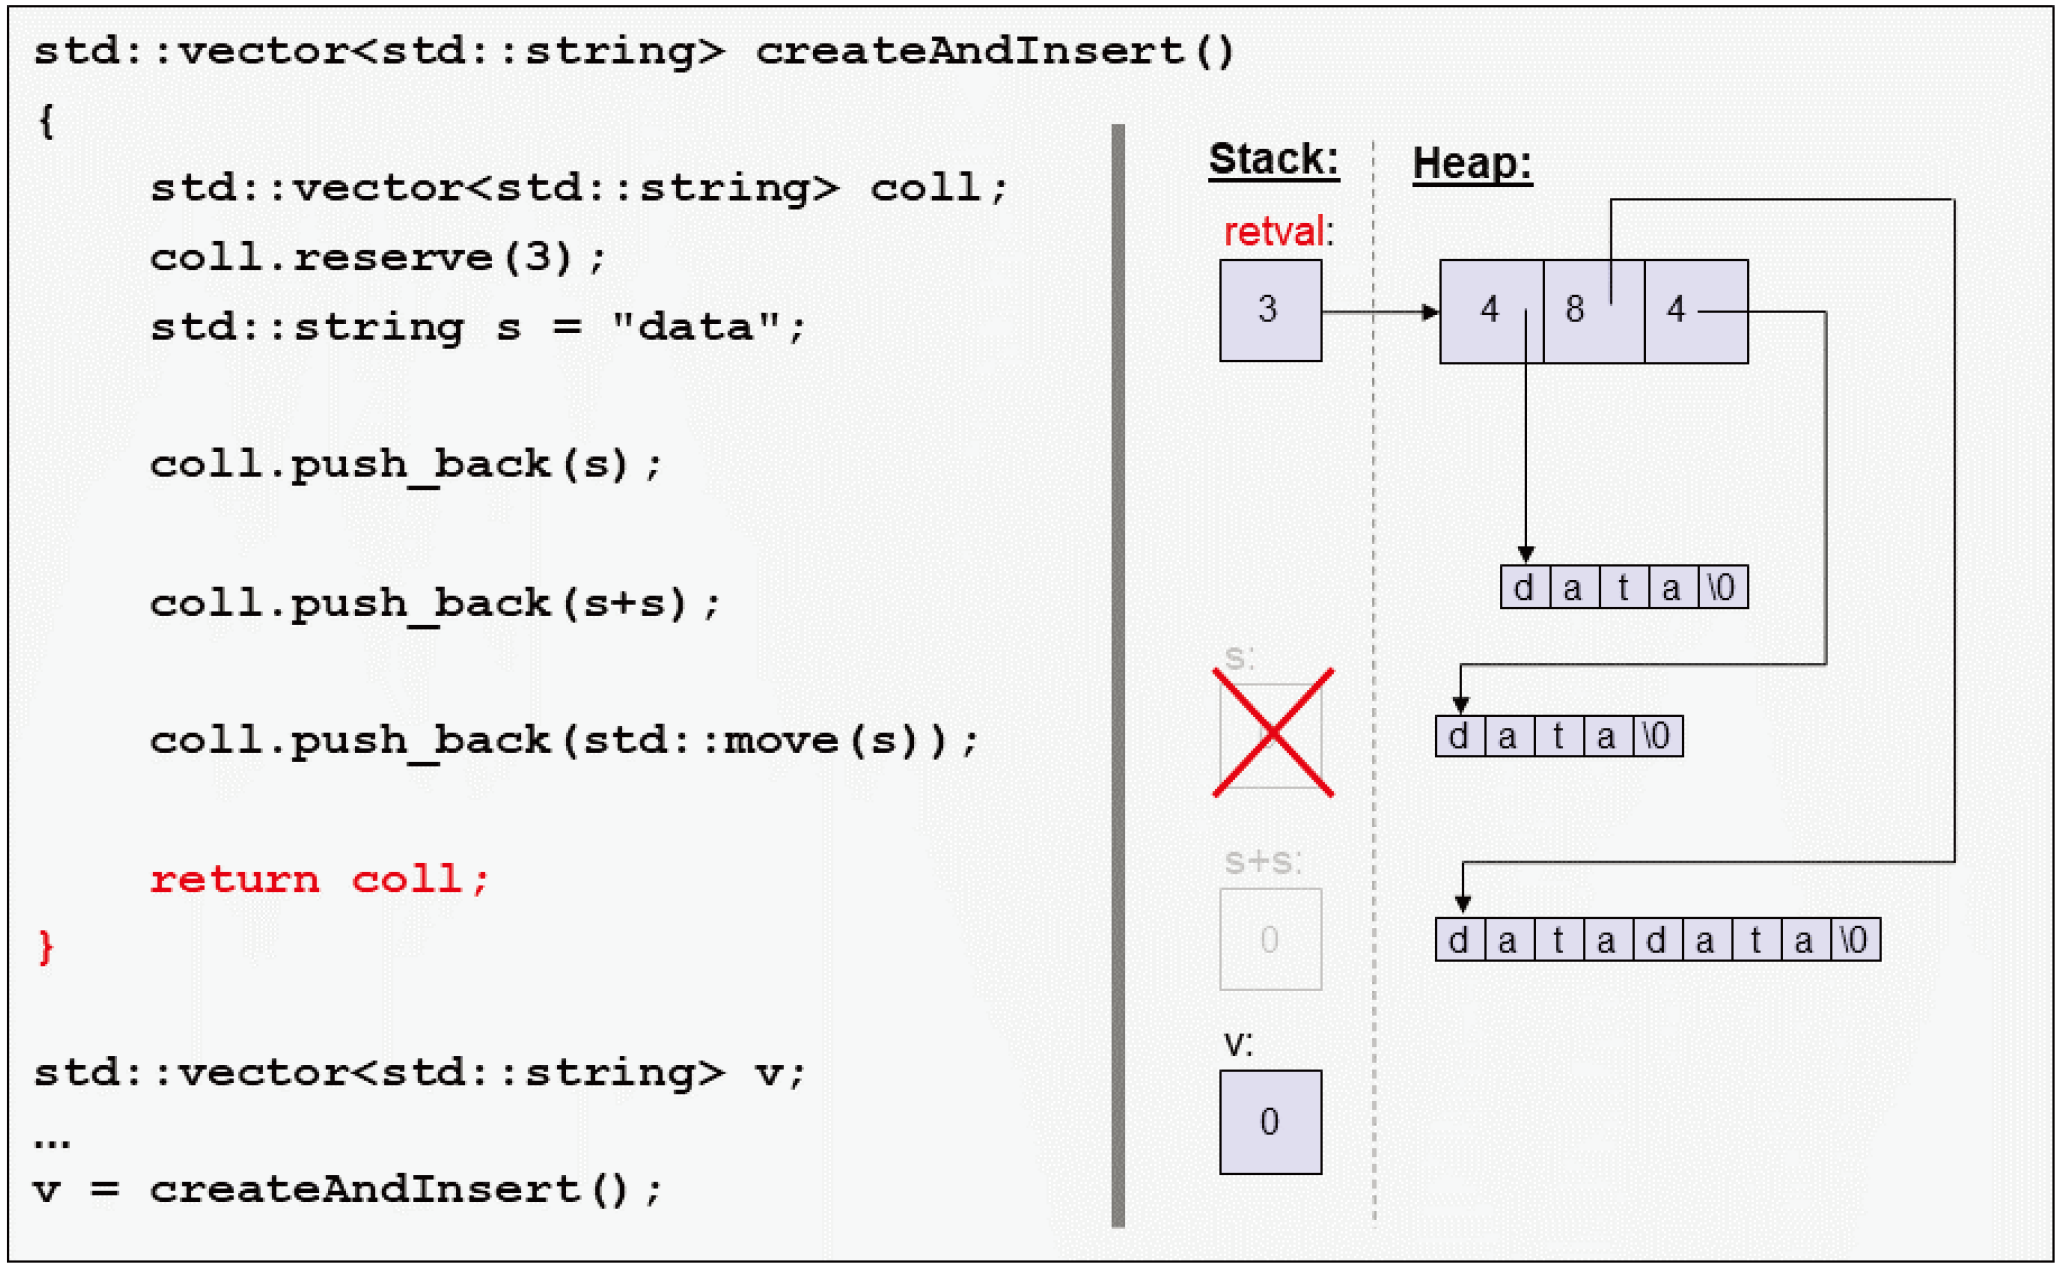
\includegraphics[width=1.0\textwidth]{content/1/chapter1/images/15}
	\end{center}
	\item 最后,我们来给\textit{v}赋值:\par
	\textit{\textbf{v = createAndInsert();}}\par
	同样可以从移动语义中获益:必须从一个即将销毁的临时返回值中复制(这里是赋值)一个值。\par
	现在,移动语义允许从源vector转移值的赋值操作符:\par
	\begin{center}
		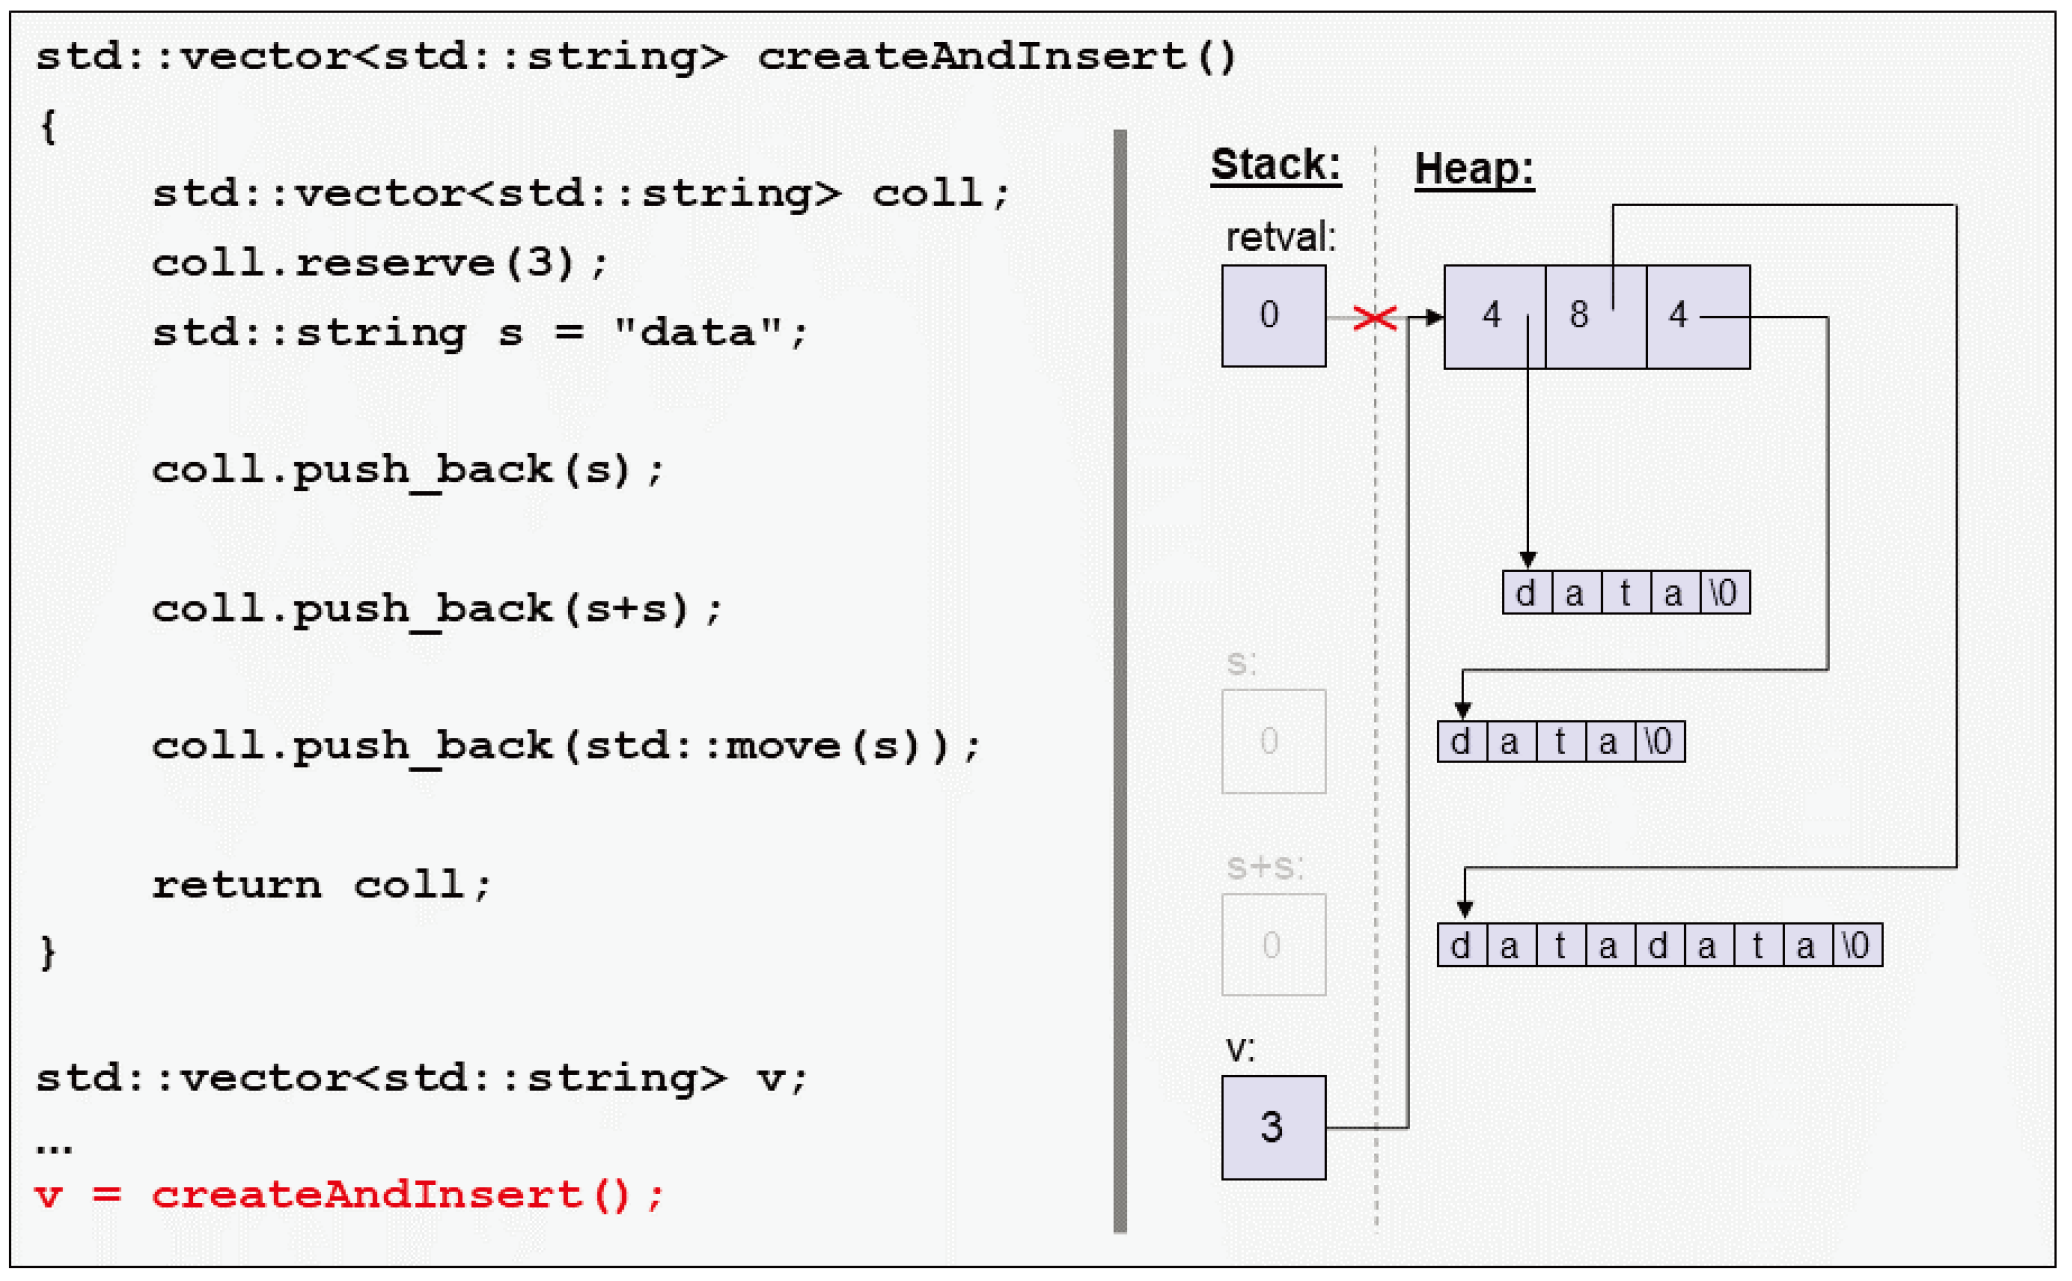
\includegraphics[width=1.0\textwidth]{content/1/chapter1/images/16}
	\end{center}
	同样,临时对象不会(部分地)销毁。它进入了某个状态,但我们不知道它的值。\par
	但是,在赋值之后,语句的末尾会销毁(修改过的)临时返回值:\par
	\begin{center}
		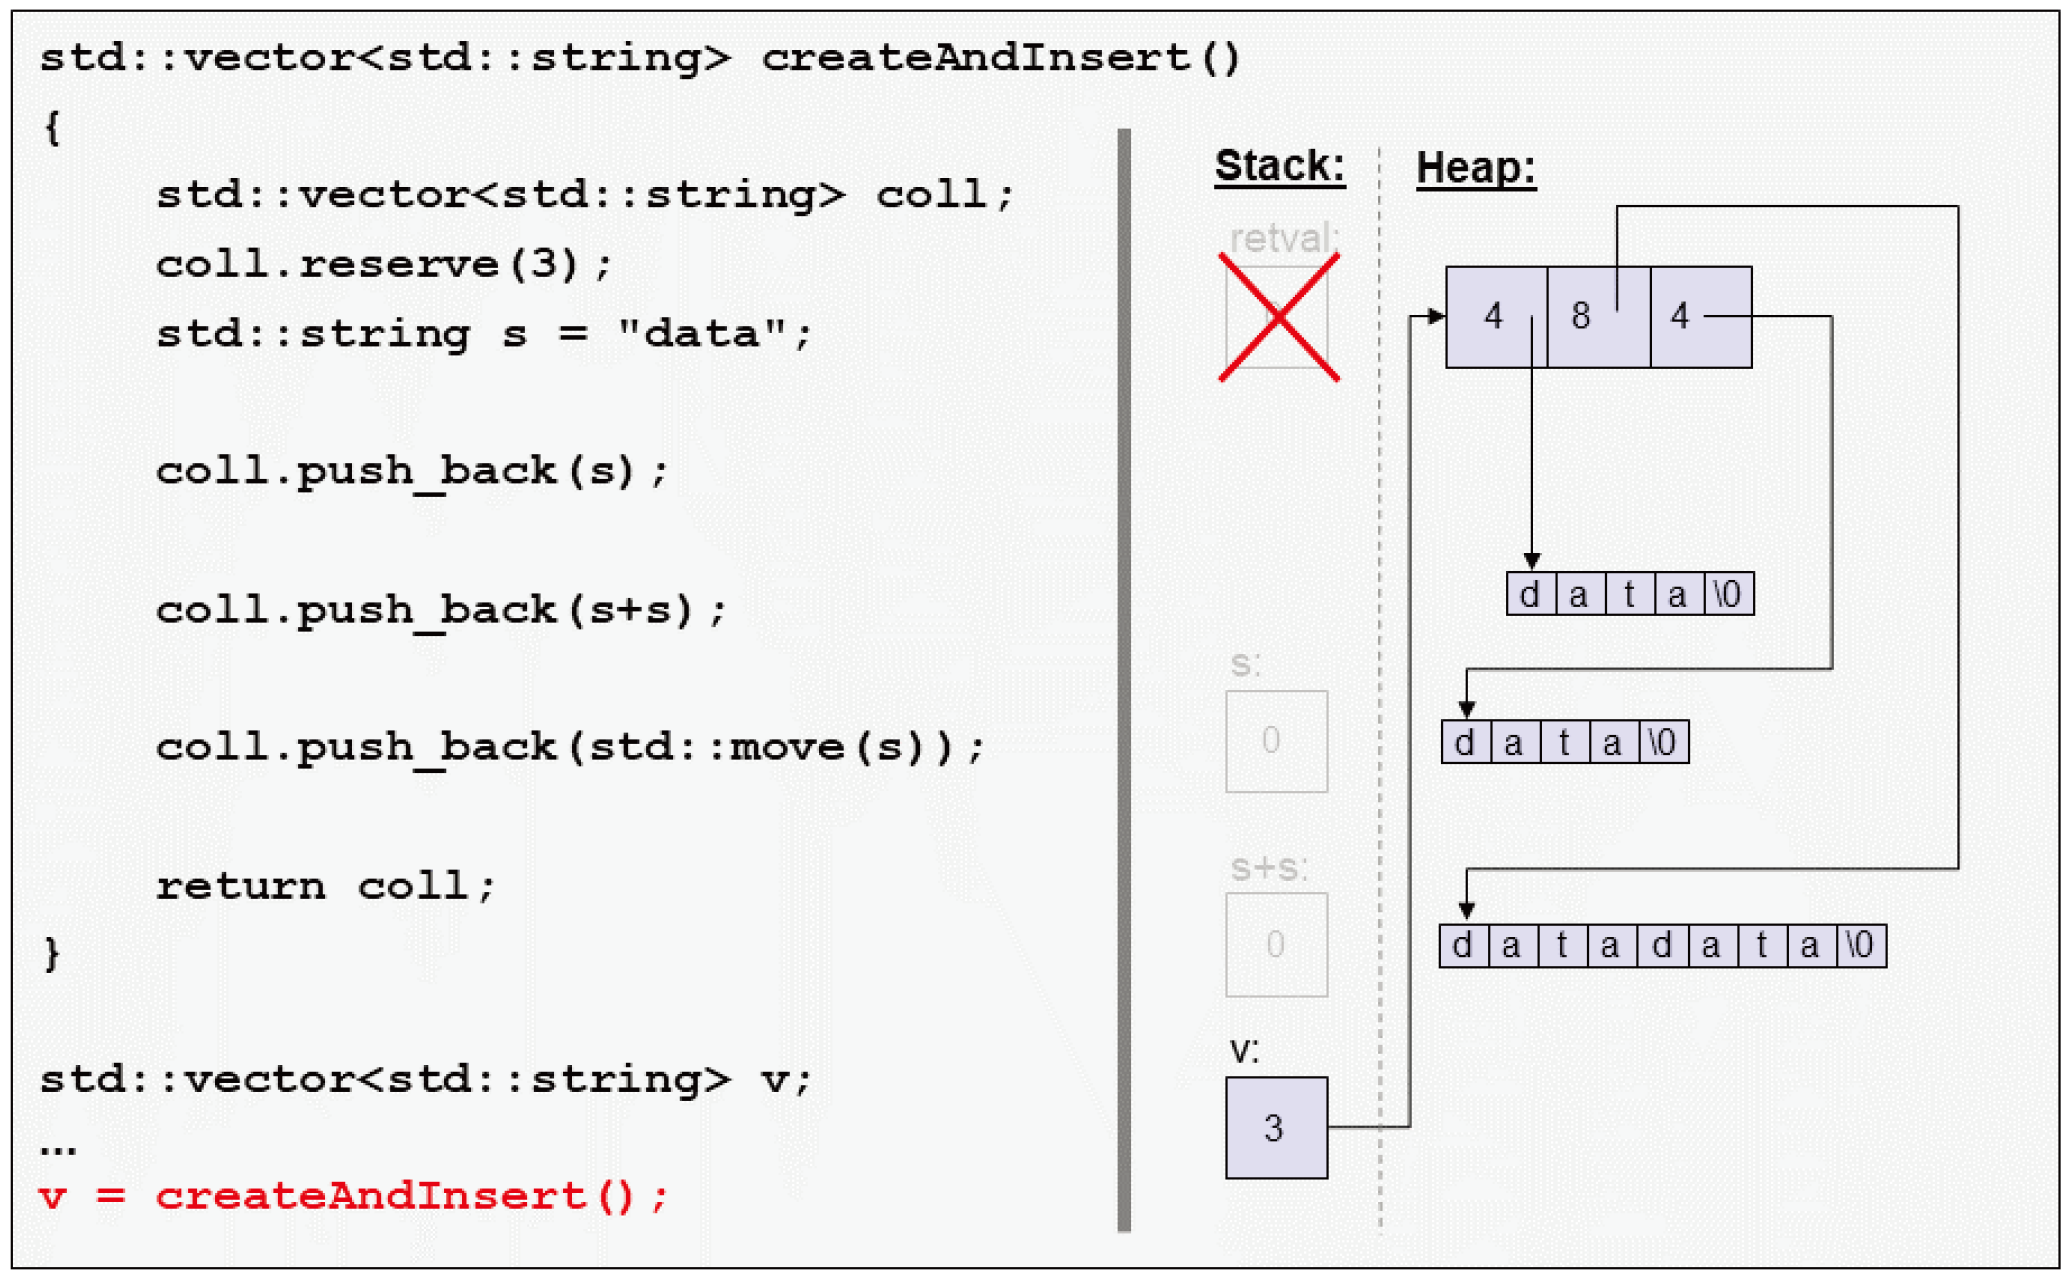
\includegraphics[width=1.0\textwidth]{content/1/chapter1/images/17}
	\end{center}
\end{itemize}

最后,和之前使用移动语义时一样,但有一些事情发生了改变:节省了6个内存分配和释放。所有不必要的内存分配不再发生:\par

\begin{itemize}
	\item 将临时对象移动插入容器
	\item 当使用\textit{std::move()}表示不再需要该值时,用于将对象移动插入容器
	\item 临时vector及其元素的分配方式
\end{itemize}

在第二种情况下,优化是在我们的帮助下完成的。通过添加\textit{std::move()},说明不再需要\textit{s}的值。所有其他优化都生效了,因为编译器知道对象即将销毁,所以编译器也可以使用移动语义的优化实现。\par

这意味着返回字符串向量,并将其赋值给一个现有向量不再是性能问题。我们可以像使用整型一样使用字符串向量,从而获得更好的性能。在实践中,用移动语义重新编译代码可以将速度提高10\%到40\%(取决于现有代码的难易程度)。\par


























